\documentclass[a4paper]{scrartcl}
\usepackage[cm]{fullpage}
\usepackage{amsmath, amssymb, esint}
\usepackage{siunitx}

\usepackage{tikz, pgfplots}
\pgfplotsset{compat = 1.12}

\begin{document}

\title{PHYS3117: Scanning Electron Microscopy}
\author{Donny Yang \\ z3470068}
\date{2017-09-14}
\maketitle

\section{Materials and Methods}
\begin{figure}
    \centering
    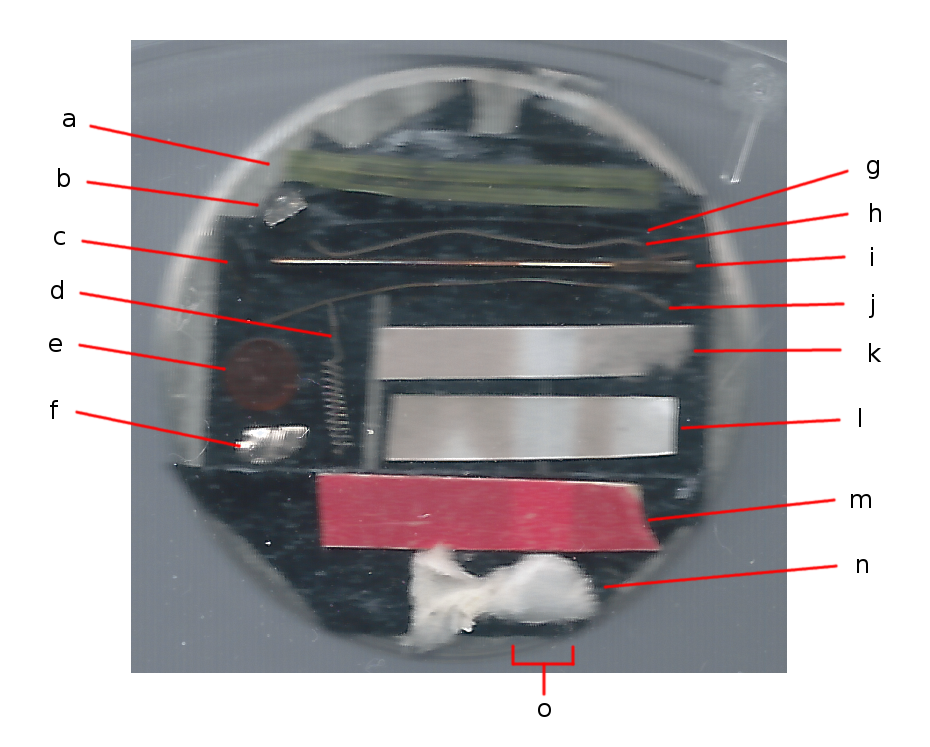
\includegraphics[width = 10cm]{samples.png}
    \caption{Poorly scanned image of the sample stub. Descriptions of each element is in Table \ref{tab:samples}.}
    \label{fig:samples}
\end{figure}
\begin{table}
    \centering
    \begin{tabular}{c | l}
    \# & Material \\
    \hline
    a & Generic lawn grass \\
    b & \SI{60}{\watt} light bulb bayonet \\
    c & \SI{60}{\watt} light bulb glass \\
    d* & \SI{100}{\watt} light bulb filament \\
    e & GCu200 copper grid \\
    f & \SI{60}{\watt} light bulb contact pad \\
    g & Human head hair \\
    h & \SI{60}{\watt} light bulb filament \\
    i & \SI{60}{\watt} light bulb electrode \\
    j & \SI{60}{\watt} light bulb filament support \\
    k & Grid/graph paper \\
    l* & Plastic backing of sticky tape \\
    m* & AMF ticket \\
    n & Styrofoam \\
    o* & Strip that was left uncoated with the carbon
    \end{tabular}
    \caption{List of the samples prepared for the microscope. An image of them is in Figure \ref{fig:samples}. (*) indicates that while the sample was prepared, they are not referred to in this report.}
    \label{tab:samples}
\end{table}

Please refer to the student notes of the experiment.

The light bulb's filament was measured to have a resistance of \SI{65}{\ohm}. Since this is a \SI{60}{\watt} light bulb, this value should increase to \SI{882}{\ohm} when operating under \SI{230}{\volt} electricity.

A copper grid, parts of a light bulb, various types of paper, human hair, grass and styrofoam were prepared on the sample stub, as shown in Figure \ref{fig:samples} and Table \ref{tab:samples}.

They were then coated with a thin carbon layer, before being placed into the microscope.

All X-ray measurements were done with a \SI{11}{\milli\metre} working distance, at \SI{30}{\kilo\volt}, and at \(>5000 \times\) magnification.

All errors in the compositional analysis results are their 1-\(\sigma\) errors.

\section{Results}
\subsection{Light Bulb Parts}
\subsubsection{Secondary Electron Images}
\begin{figure}
    \centering
    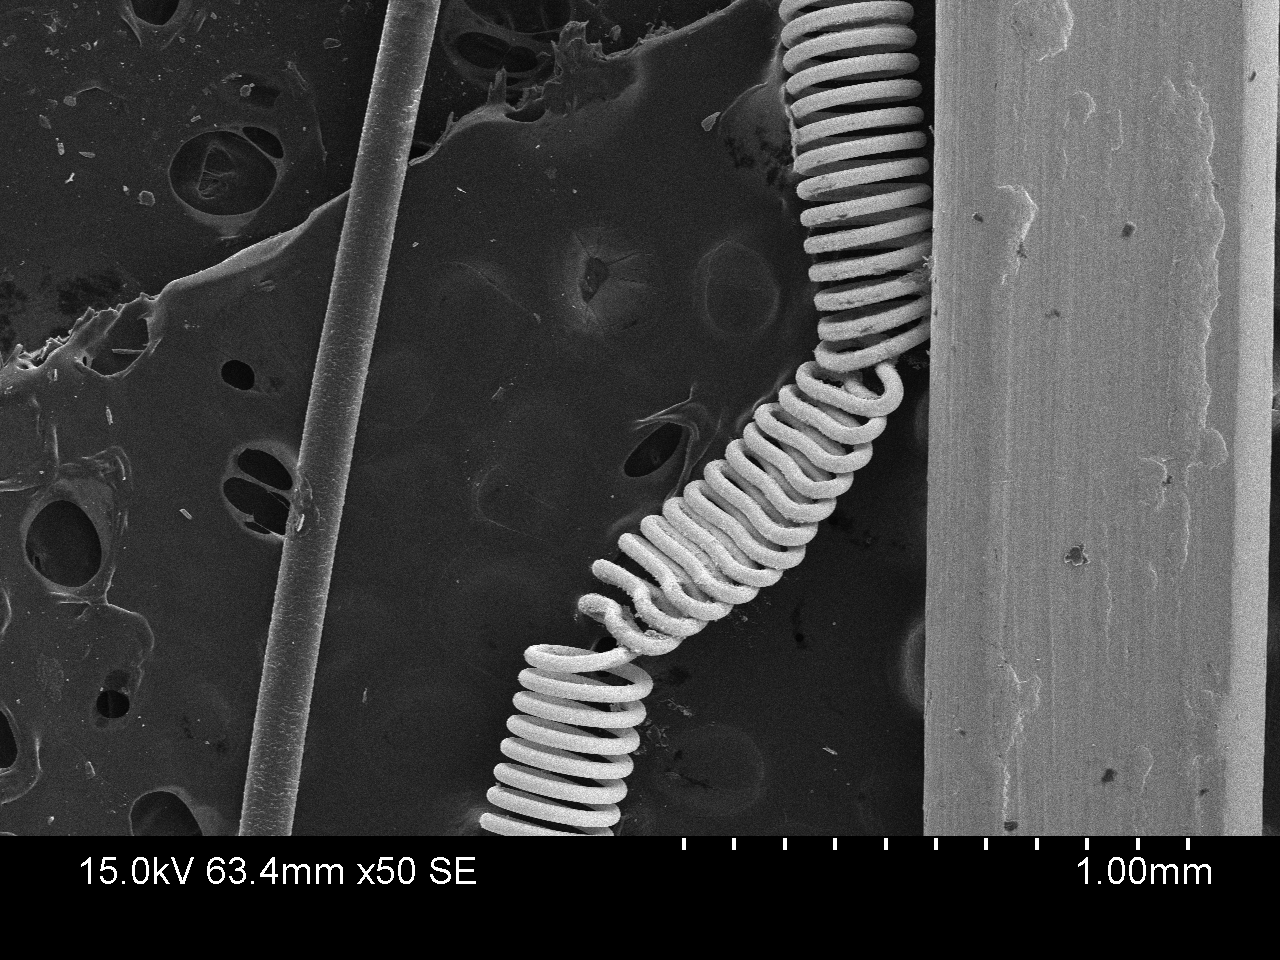
\includegraphics[width = 15cm]{measurements/SE-filament-low.png}
    \caption{Zoomed out view of the light bulb filament, of which half is where the electrode clamped on to it}
    \label{fig:se-filament-low}
\end{figure}
\begin{figure}
    \centering
    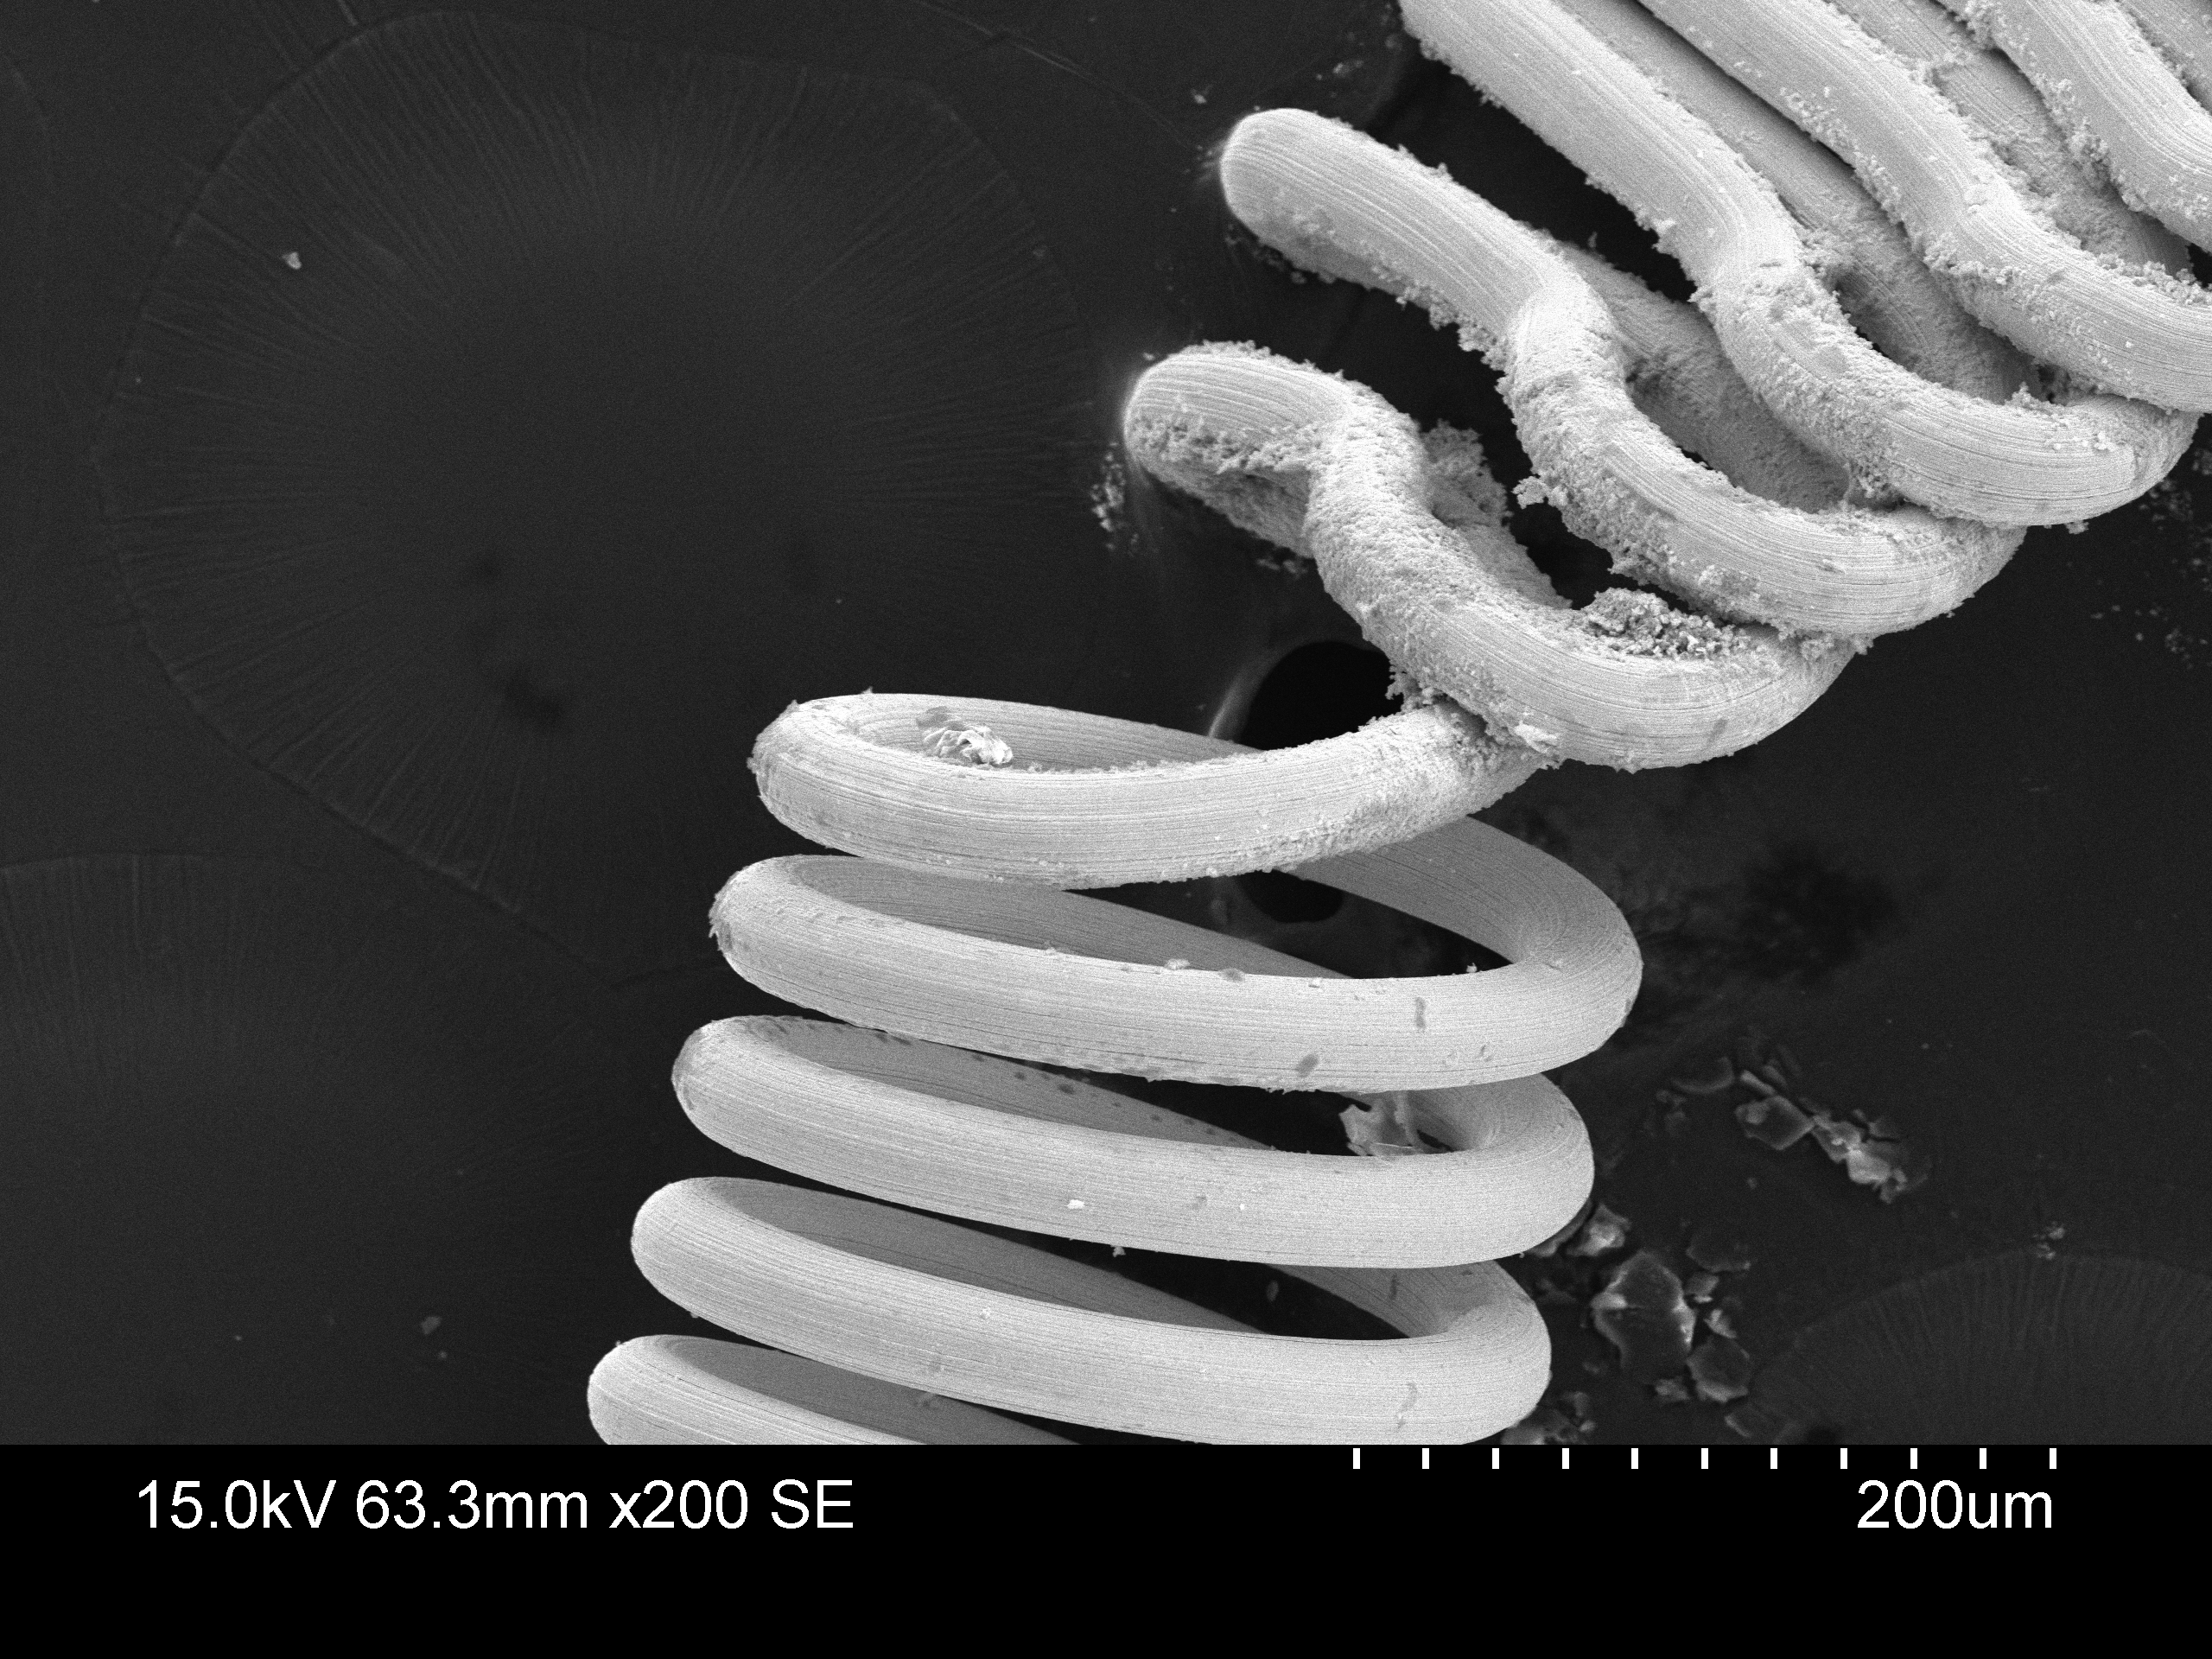
\includegraphics[width = 15cm]{measurements/SE-filament-medium.png}
    \caption{Same as Figure \ref{fig:se-filament-low}, but zoomed in}
    \label{fig:se-filament-medium}
\end{figure}
\begin{figure}
    \centering
    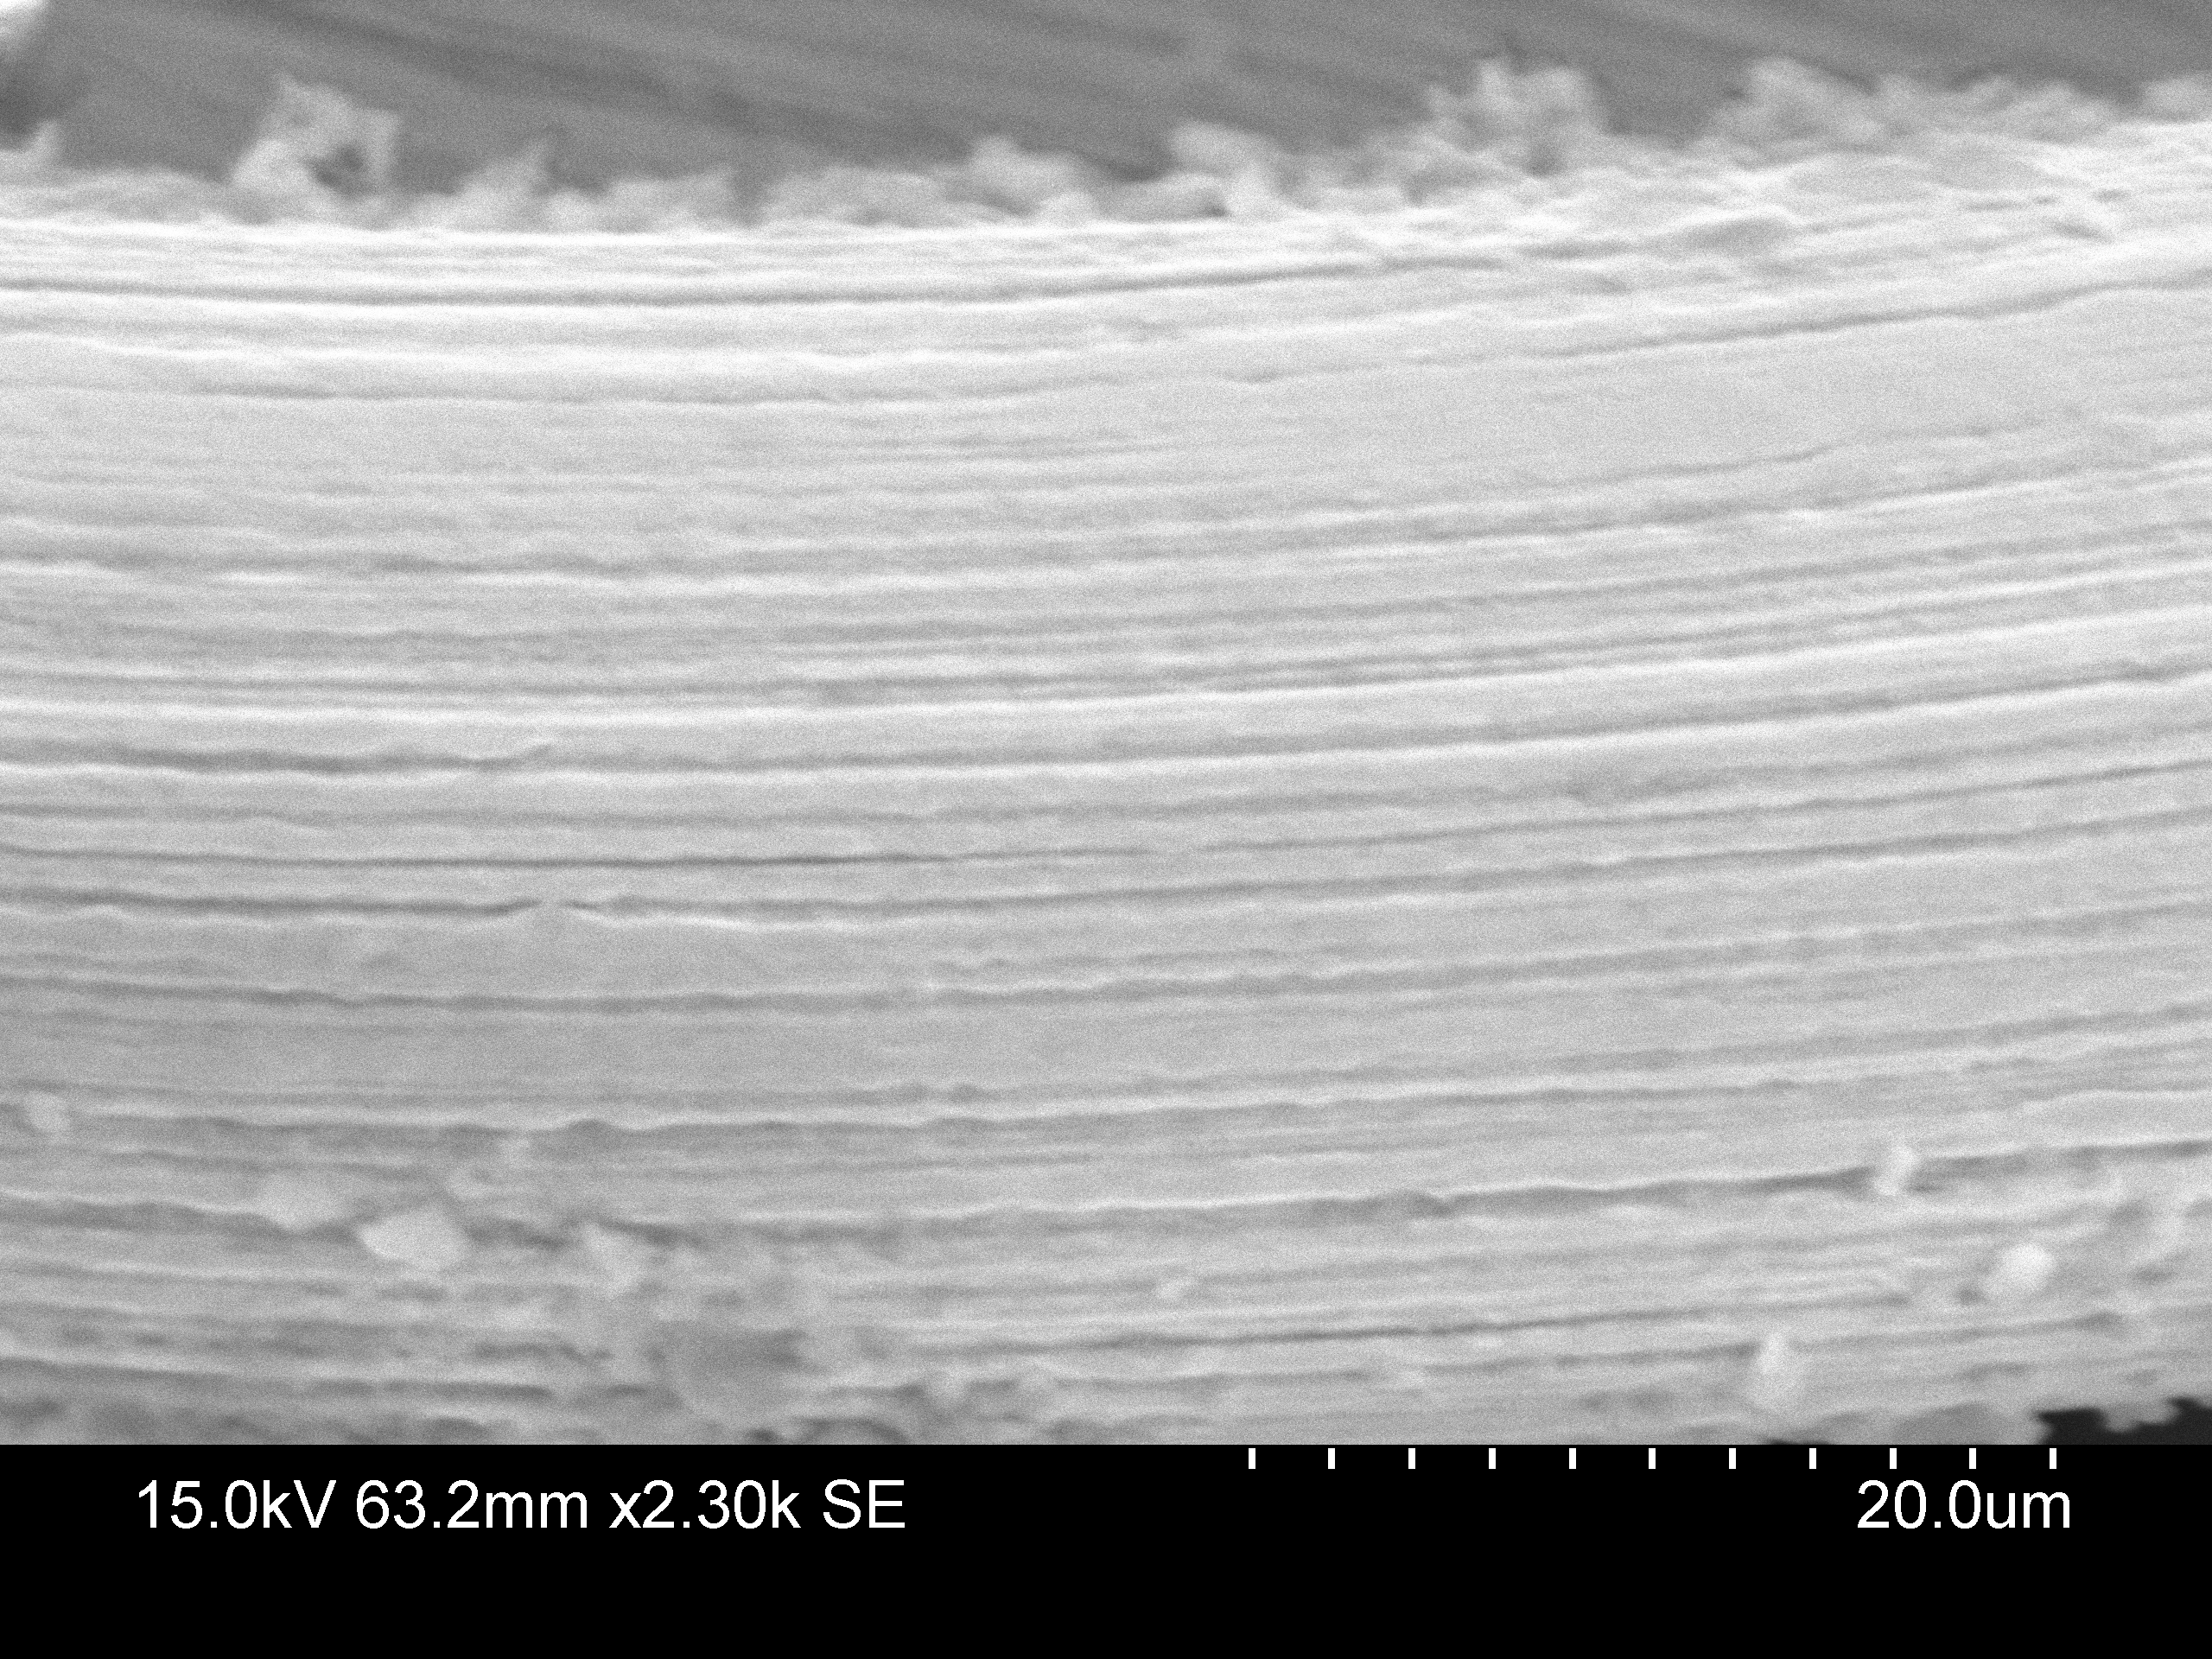
\includegraphics[width = 15cm]{measurements/SE-filament-high.png}
    \caption{Same as Figure \ref{fig:se-filament-medium}, but zoomed in on a single turn of the coil}
    \label{fig:se-filament-high}
\end{figure}

Only images of the filament were taken, since all the other parts were visually featureless. They can be seen in Figures \ref{fig:se-filament-low}, \ref{fig:se-filament-medium} and \ref{fig:se-filament-high}.

From Figure \ref{fig:se-filament-medium}, one can measure the wire diameter to be \(\frac{r_w}{2} = \SI{32 \pm 3}{\micro\metre}\) and coil diametre to be \(\frac{r_c}{2} = \SI{232 \pm 5}{\micro\metre}\). There also appears to be one coil per \(T = \SI{47 \pm 1}{\micro\metre}\).

Using the length of the original coil, which was measured to be \(h = \SI{62 \pm 1}{\milli\metre}\), and the coil length formula:
\[l = h \sqrt{1 + \frac{4 \pi r_c^2}{T^2}}\]
results in a total length of \SI{963 \pm 33}{\milli\metre}.

The resistivity of tungsten is \(\rho = \SI{52.8}{\nano\ohm\metre}\) at \SI{20}{\kelvin}, so the total resistance should be:
\[R = \rho \frac{l}{\pi r_w^2} \approx \SI{63 \pm 12}{\ohm}\]

Alternatively, we could turn this around and estimate \(\rho\) from our know resistances of \SI{65}{\ohm} (room temperature) or \SI{882}{\ohm} (operating). This gives estimates of \SI{54 \pm 10}{\nano\ohm\metre} at room temperature or \SI{740 \pm 140}{\nano\ohm\metre} under load.

\subsubsection{Characteristic X-rays}
\begin{figure}
    \centering
    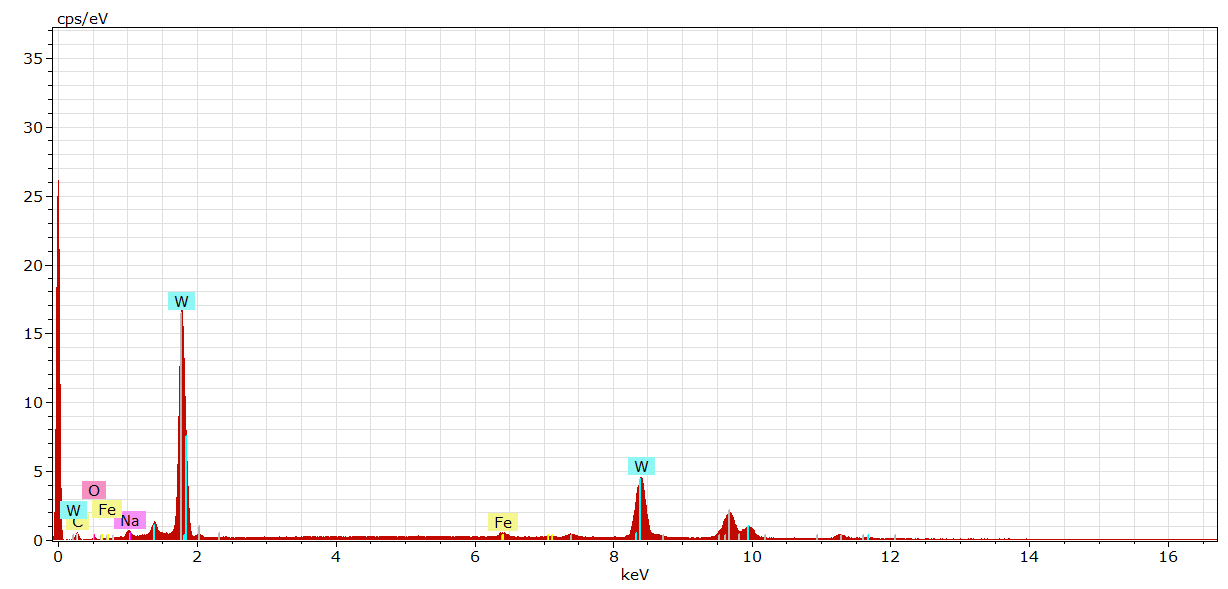
\includegraphics[width = 15cm]{measurements/XR-LB-filament.png}
    \caption{X-ray spectrum from the light bulb filament}
    \label{fig:xr-filament}
\end{figure}
\begin{table}
    \centering
    \begin{tabular}{c | c}
    Part & \si{\percent} by atom count \\
    \hline
    Filament & C \SI{53 \pm 12}{}, W \SI{27.50 \pm 0.67}{}, O \SI{9.2 \pm 2.8}{}, Na \SI{8.09 \pm 0.72}{}, Fe \SI{1.78 \pm 0.09}{} \\
    Electrode & Ni \SI{34.57 \pm 0.87}{}, C \SI{28.7 \pm 6.2}{}, Fe \SI{19.97 \pm 0.53}{}, O \SI{15.6 \pm 2.8}{}, Na \SI{1.08 \pm 0.18}{} \\
    Support & Mo \SI{45.3 \pm 1.4}{}, C \SI{42.3 \pm 8.7}{}, O \SI{12.4 \pm 3.2}{} \\
    Glass & O \SI{51.8 \pm 7.2}{}, Si \SI{24.1 \pm 1.1}{}, C \SI{10.8 \pm 2.8}{}, Na \SI{8.73 \pm 0.66}{}, Ca \SI{2.29 \pm 0.08}{}, Mg \SI{1.43 \pm 0.11}{}, Al \SI{0.78 \pm 0.07}{} \\
    Bayonet & C \SI{35.8 \pm 7.2}{}, Fe \SI{34.36 \pm 0.90}{}, O \SI{19.3 \pm 3.4}{}, Zn \SI{10.58 \pm 0.29}{} \\
    Contact Pad & C \SI{56 \pm 12}{}, Pb \SI{37.18 \pm 0.90}{}, Sn \SI{6.84 \pm 0.23}{}
    \end{tabular}
    \caption{Elemental composition of light bulb parts}
    \label{tab:xr-light-bulb}
\end{table}

Pointing the electrons at the filaments again, but this time reading the X-ray spectrum, we get Figure \ref{fig:xr-filament}. Having the raw spectrum by itself isn't very useful -- we would rather want to figure out the elemental composition from this spectrum. This can be done automatically by the computer software (which mostly boils down to finding the right combination of elemental x-ray lines that form the measured spectrum), so from this point on we only produce the result of this compositional analysis.

For each light bulb component, their compositional analysis results can be seen in Table \ref{tab:xr-light-bulb}.

\subsection{Copper Grid}
\begin{figure}
    \centering
    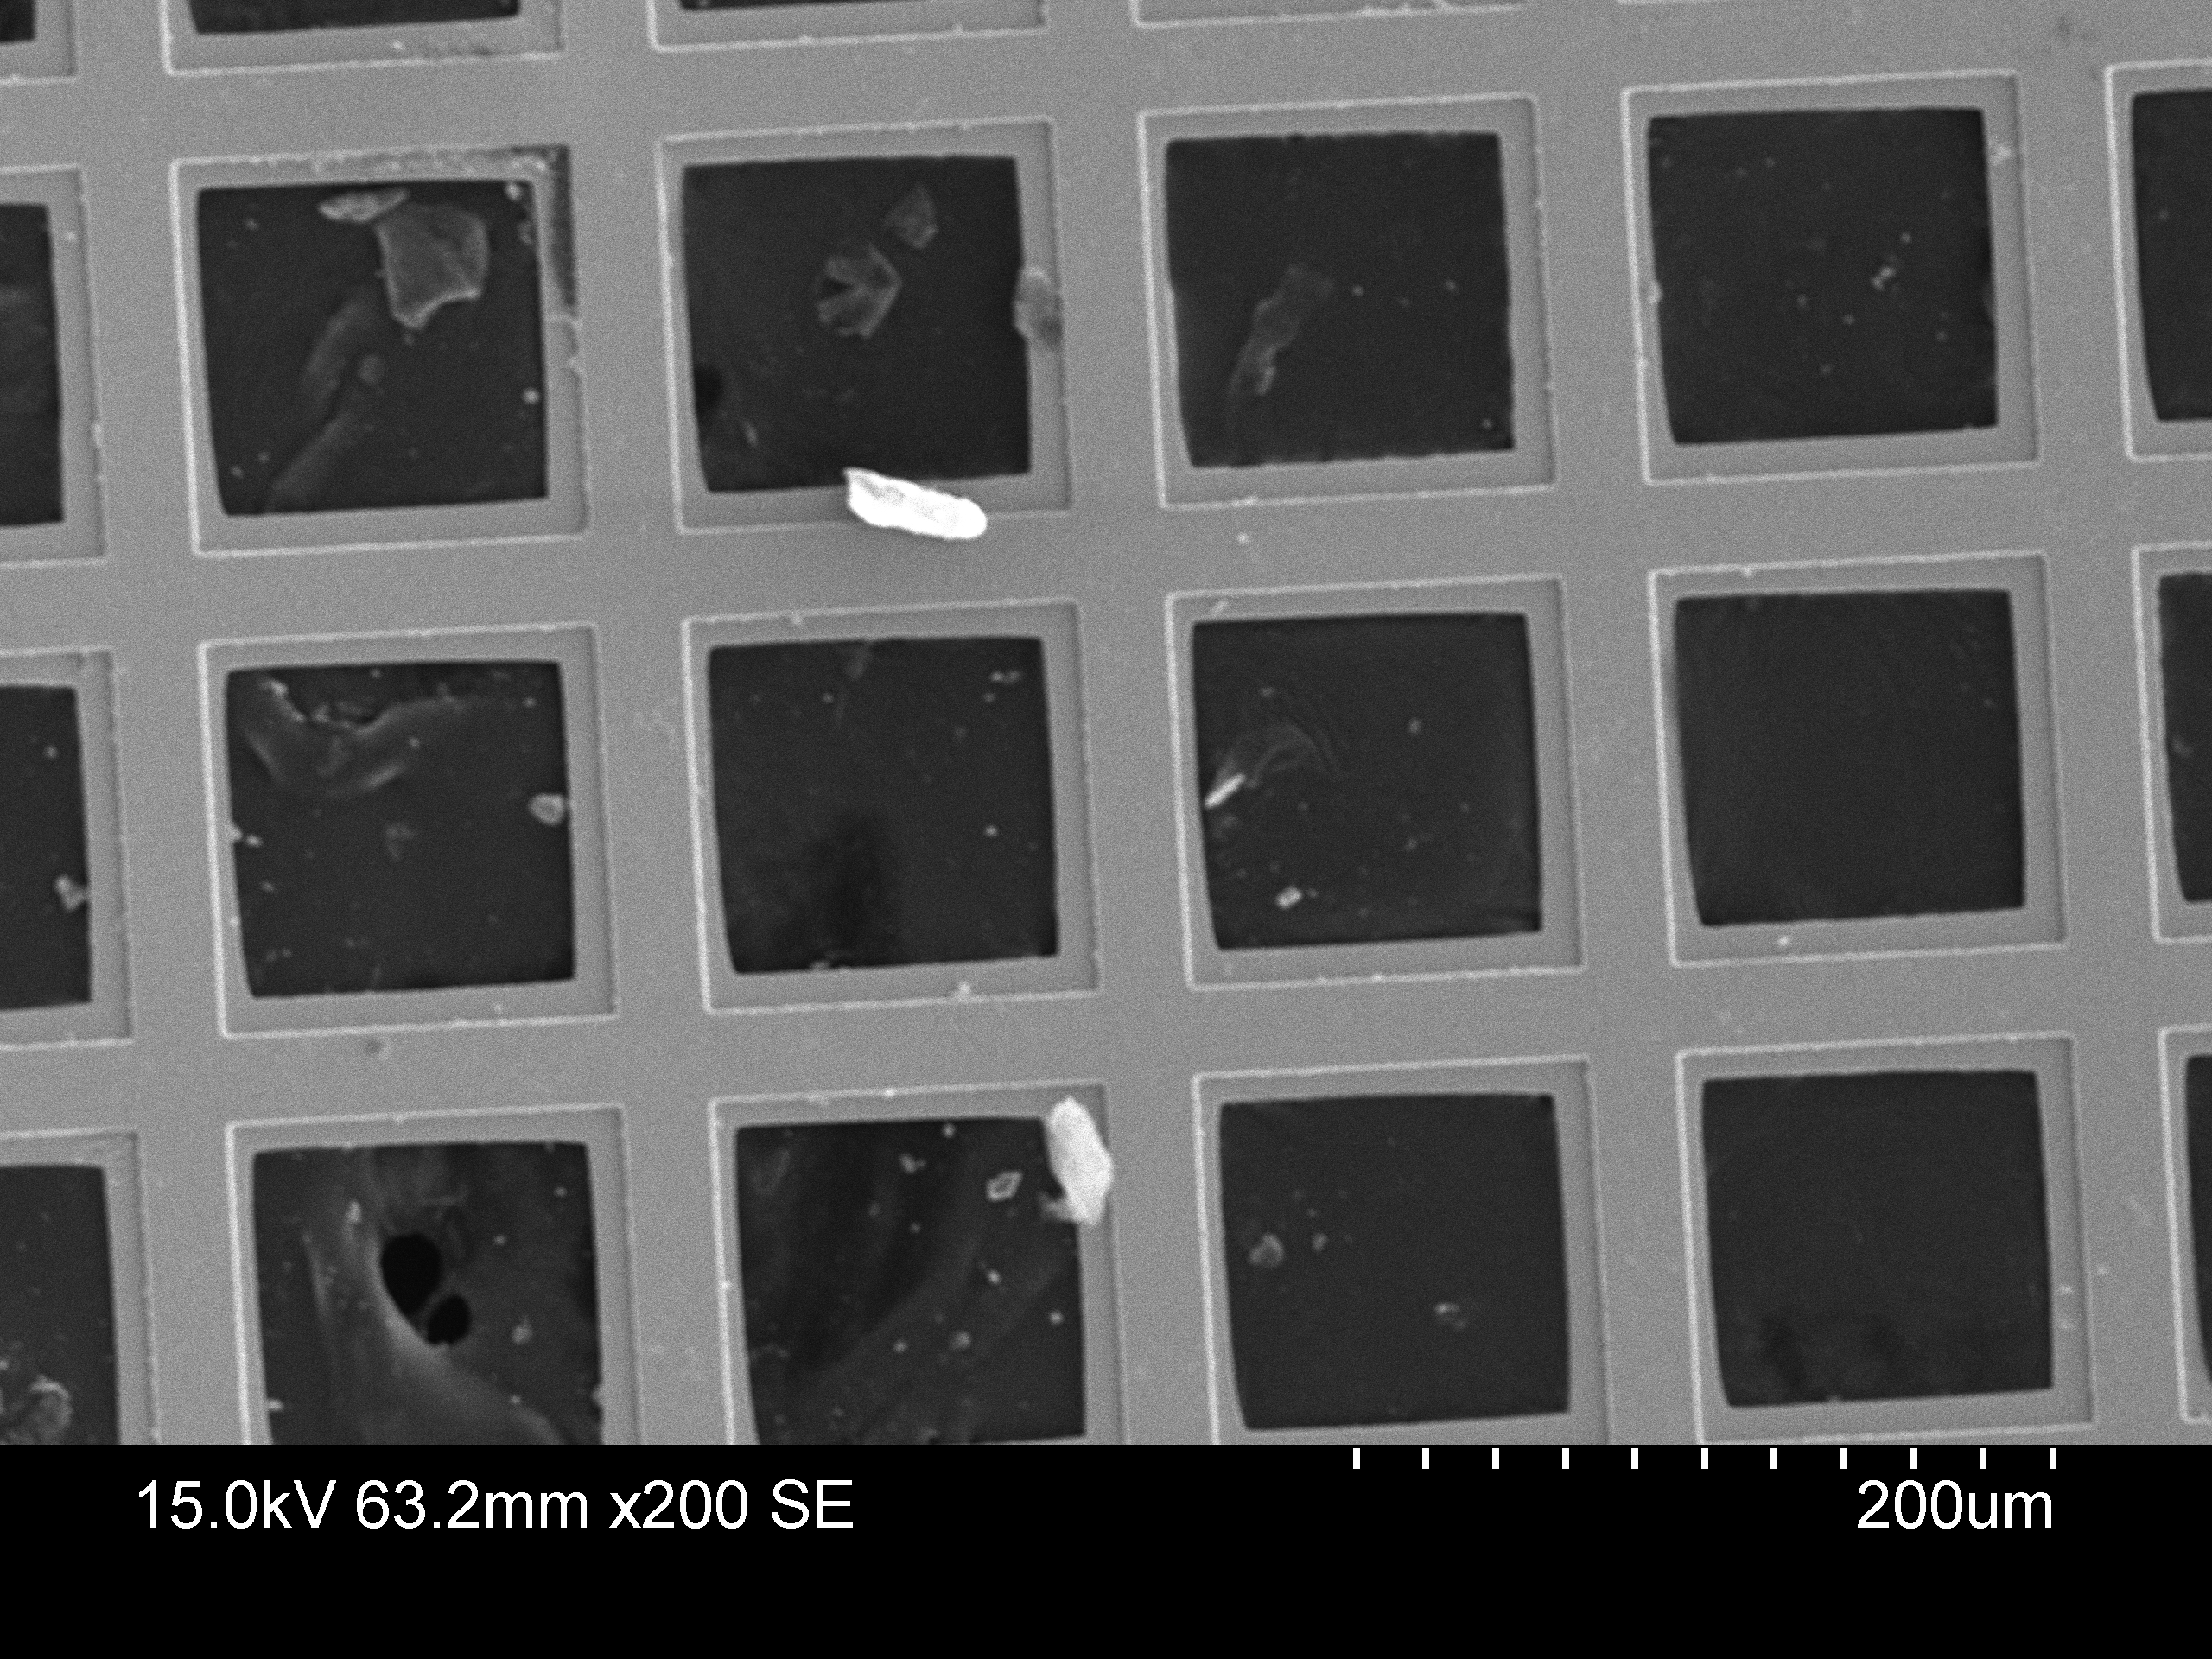
\includegraphics[width = 15cm]{measurements/SE-copper-grid.png}
    \caption{The copper grid's secondary electron image}
    \label{fig:se-copper-grid}
\end{figure}

The copper grid's secondary electron image is shown in Figure \ref{fig:se-copper-grid}, with its compositional analysis producing: Cu \SI{67.1 \pm 1.6}{\percent}, C \SI{32.9 \pm 7.3}{\percent} by atom count.

Using the scale shown on the image, each grid element pitch is about \SI{139 \pm 1}{\micro\metre} wide and tall.

\subsection{Paper}
\begin{figure}
    \centering
    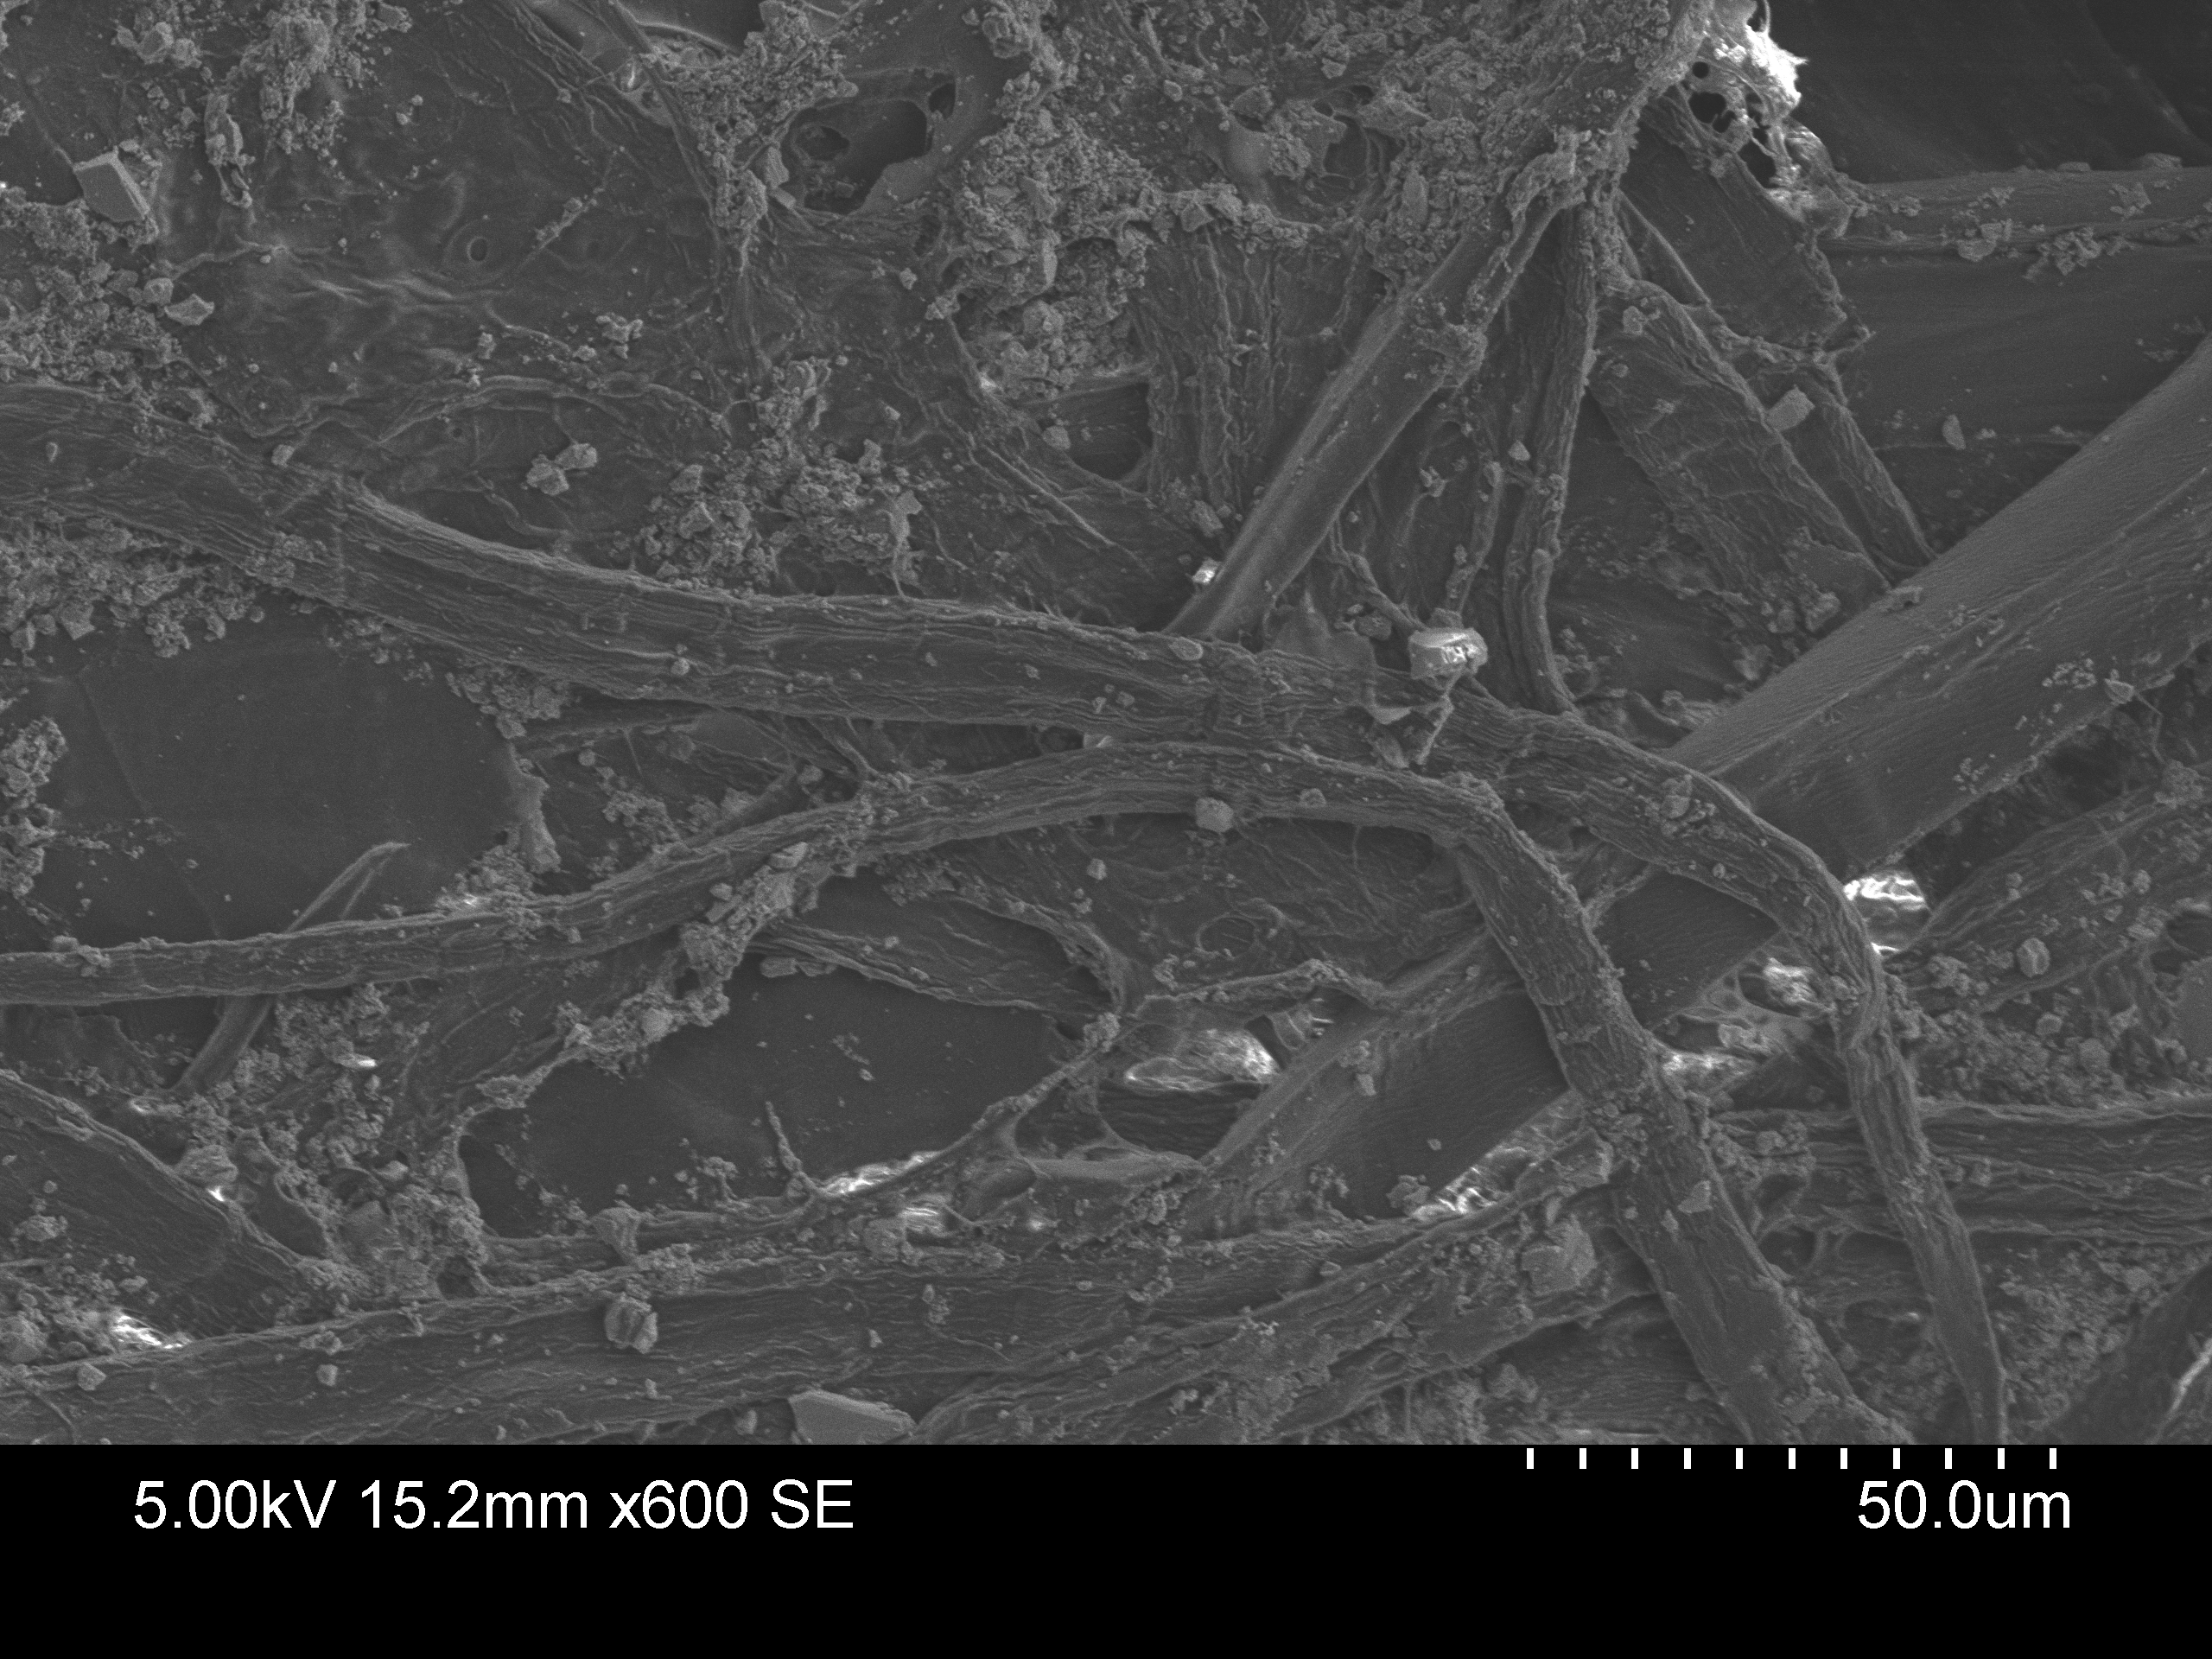
\includegraphics[width = 15cm]{measurements/SE-paper-5kV.png}
    \caption{The grid paper's secondary electron image with \SI{5}{\kilo\volt} electrons}
    \label{fig:se-paper-5kV}
\end{figure}
\begin{figure}
    \centering
    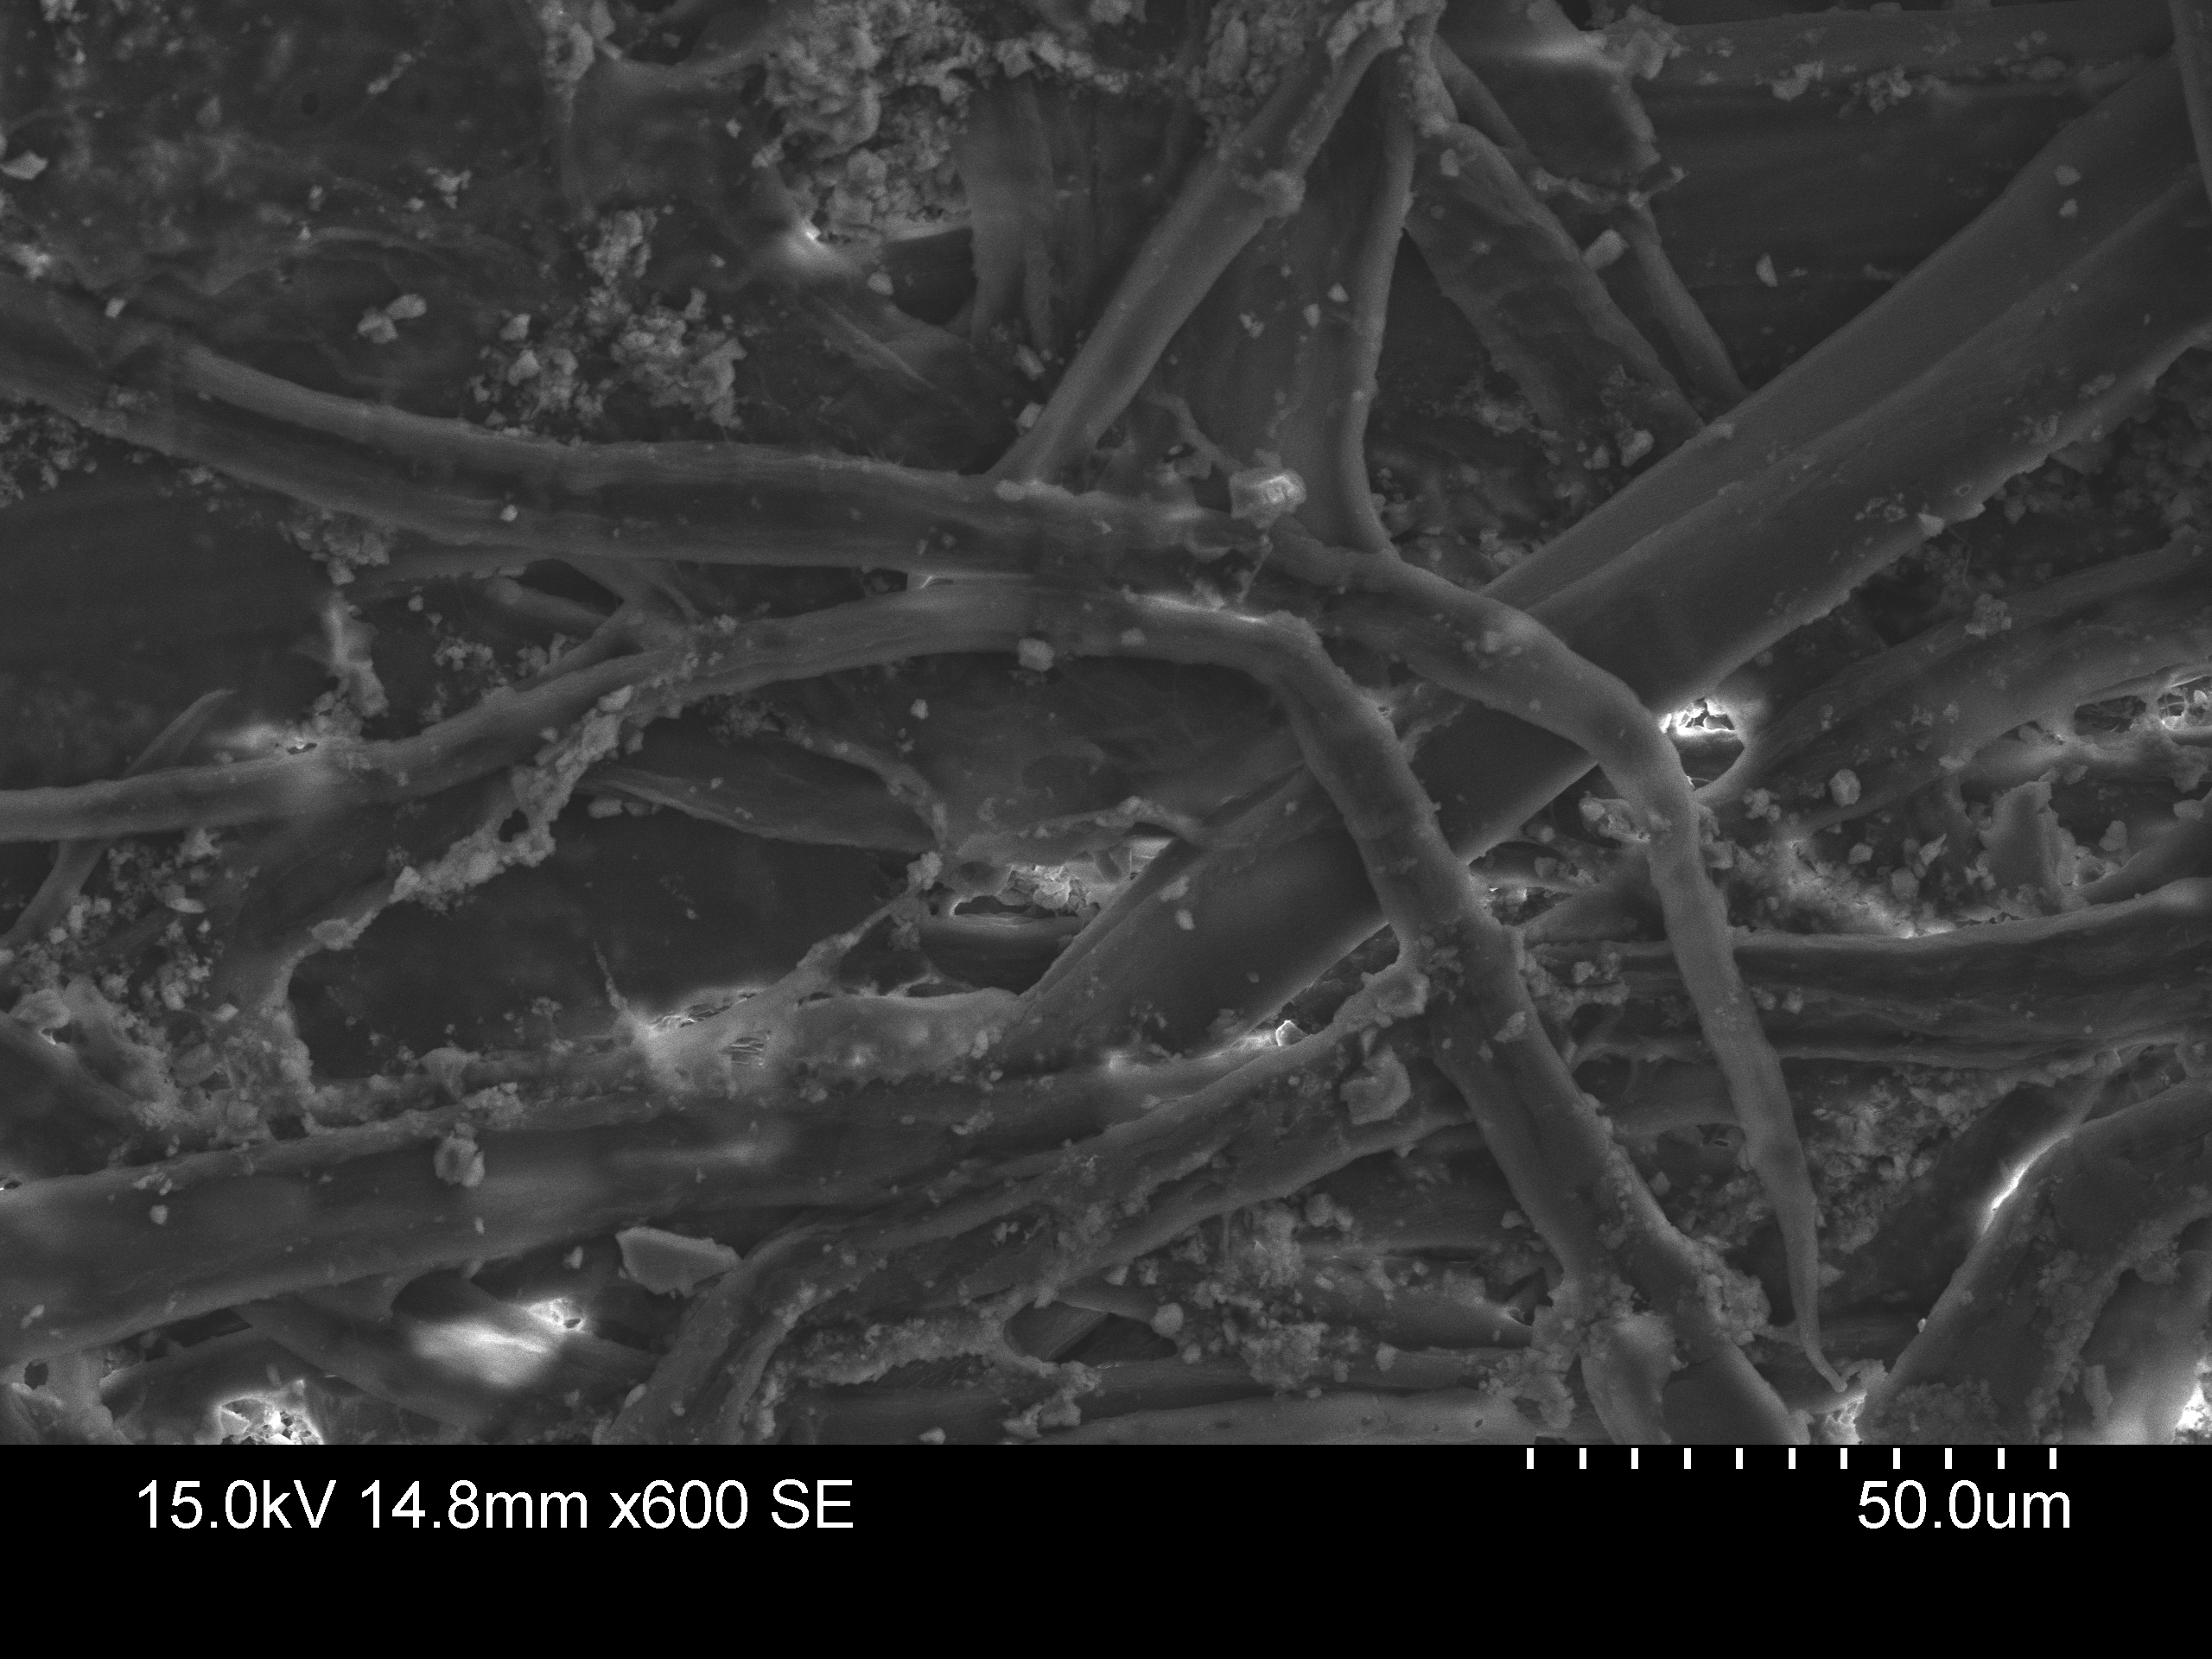
\includegraphics[width = 15cm]{measurements/SE-paper-15kV.png}
    \caption{Same as Figure \ref{fig:se-paper-5kV}, but with \SI{15}{\kilo\volt} electrons}
    \label{fig:se-paper-15kV}
\end{figure}
\begin{figure}
    \centering
    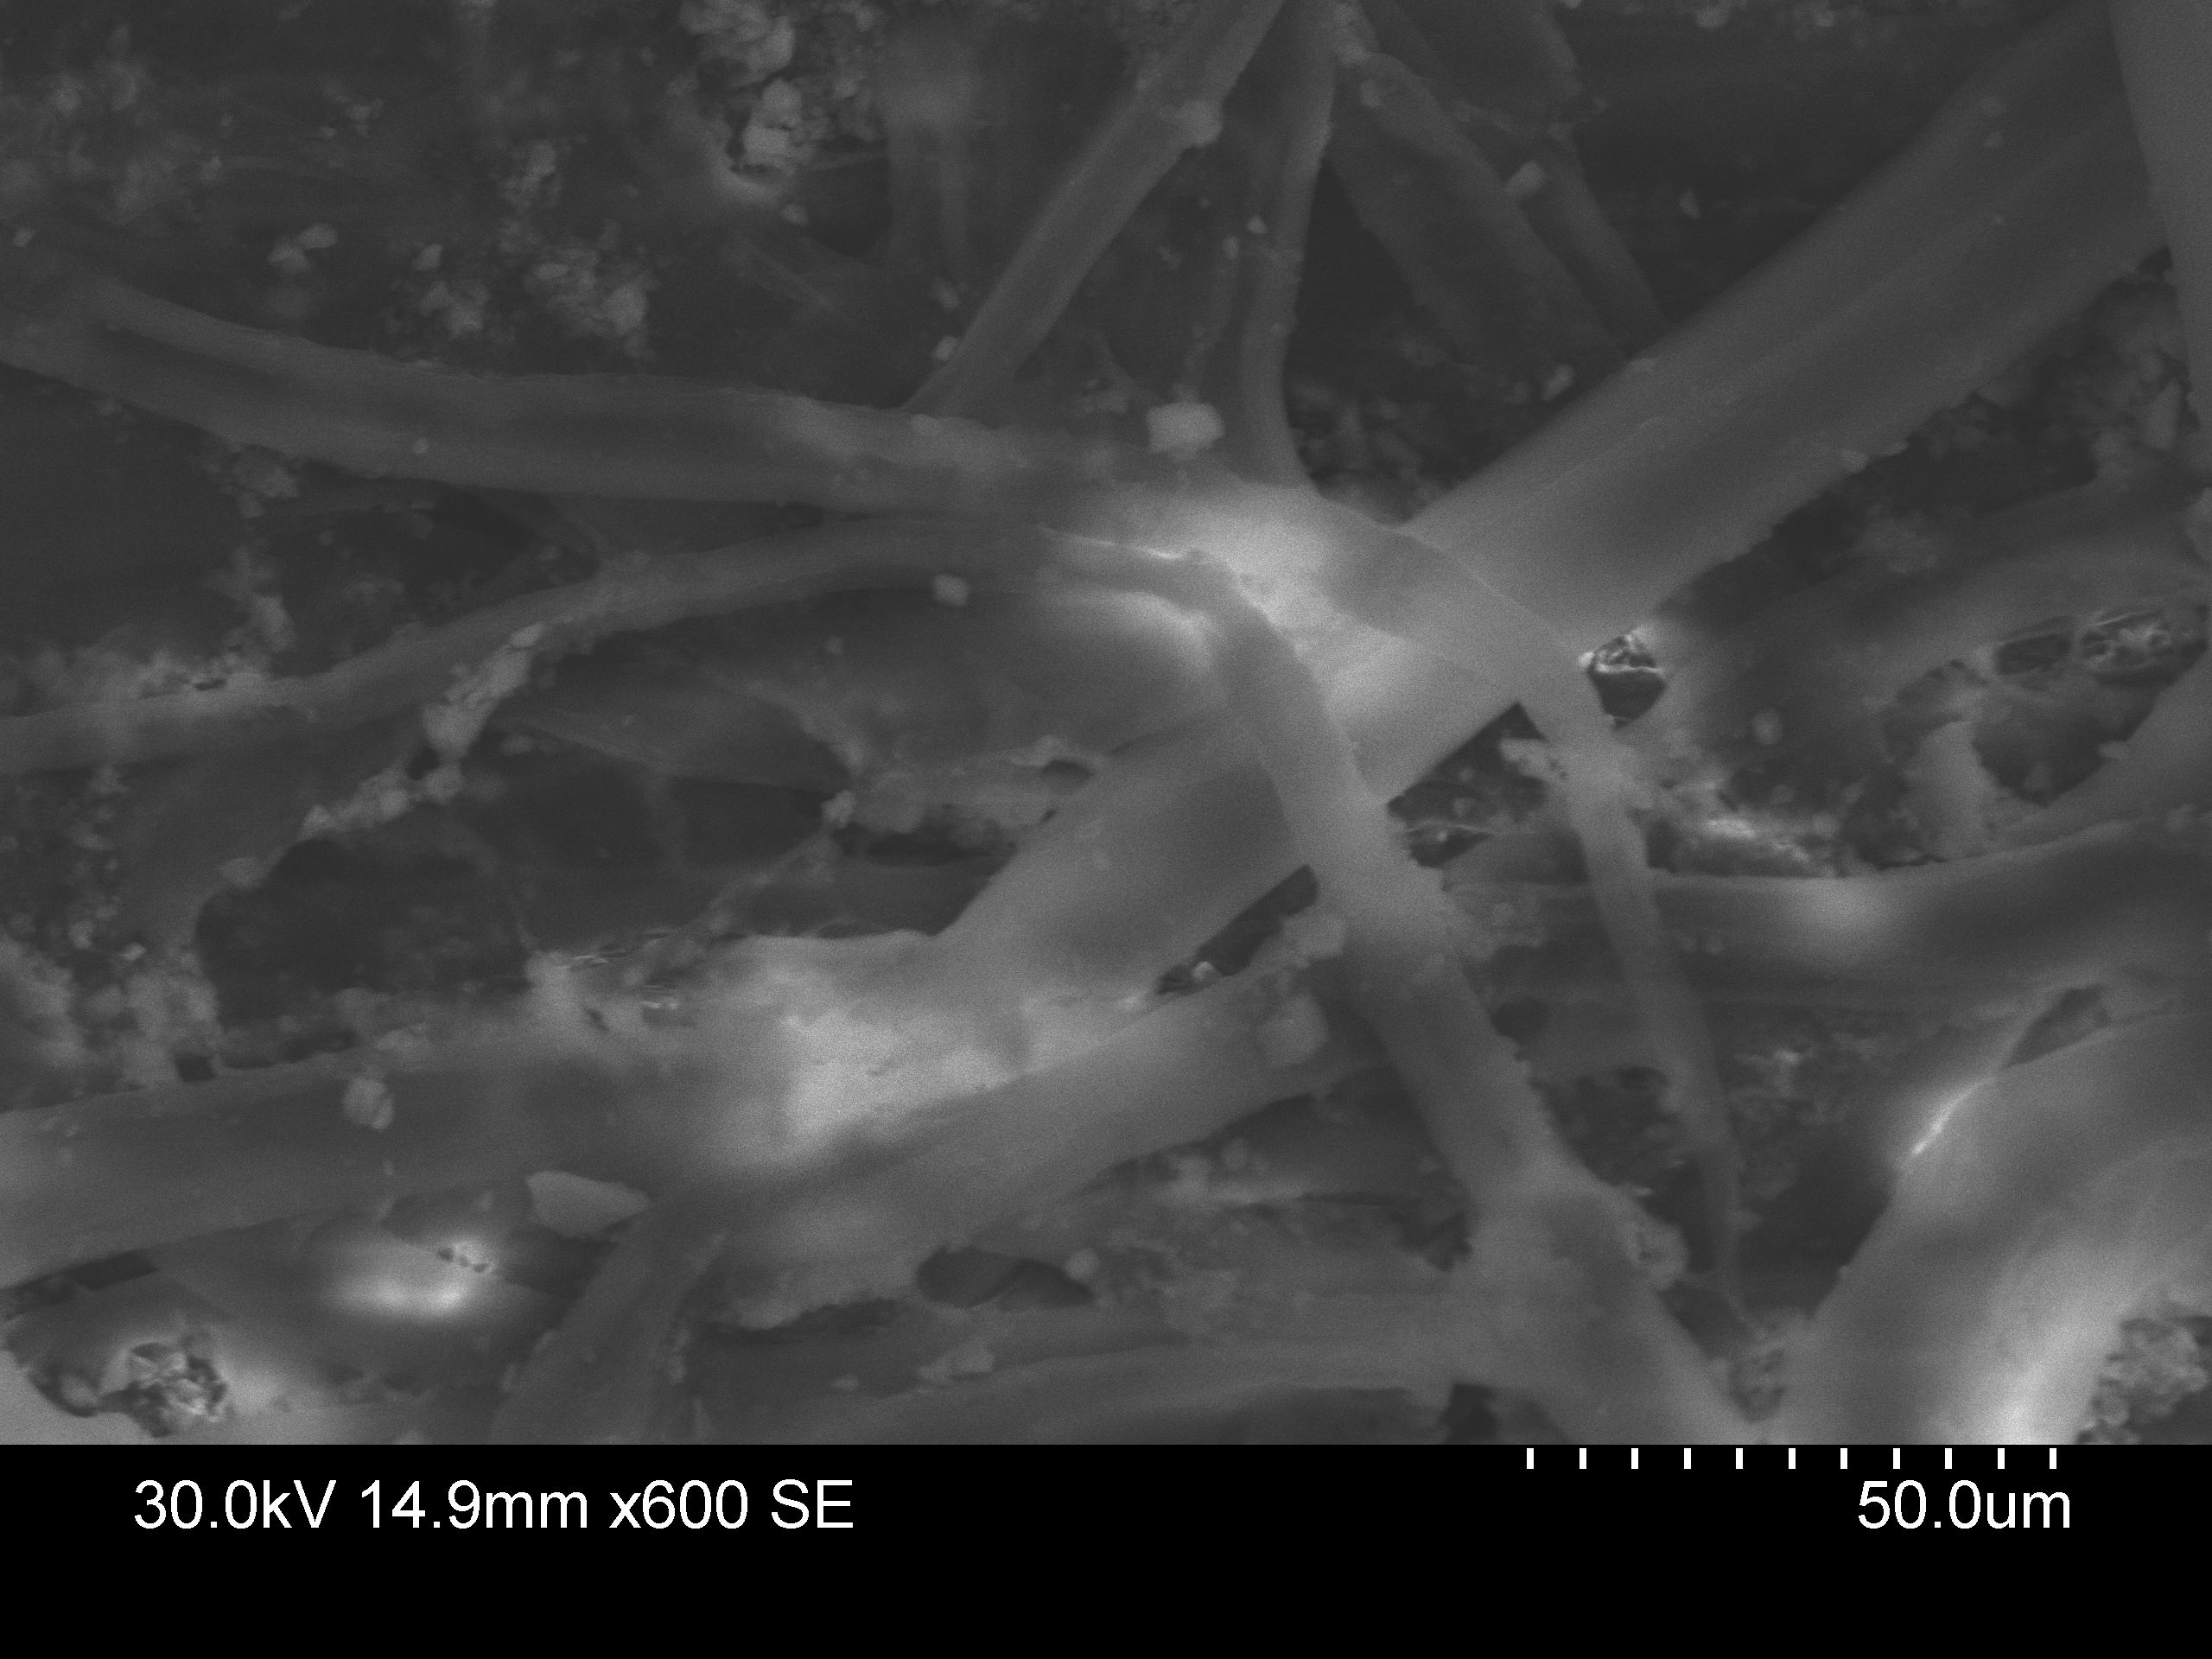
\includegraphics[width = 15cm]{measurements/SE-paper-30kV.png}
    \caption{Same as Figure \ref{fig:se-paper-5kV}, but with \SI{30}{\kilo\volt} electrons}
    \label{fig:se-paper-30kV}
\end{figure}

For the paper, we chose to only use the grid paper since it has the most interesting structure (the others turned out to be just be a boring flat plane). This time, we scanned the same area, but with different electron energies, producing the images in Figures \ref{fig:se-paper-5kV}, \ref{fig:se-paper-15kV} and \ref{fig:se-paper-30kV}.

\subsection{Other Organic Material}
\begin{figure}
    \centering
    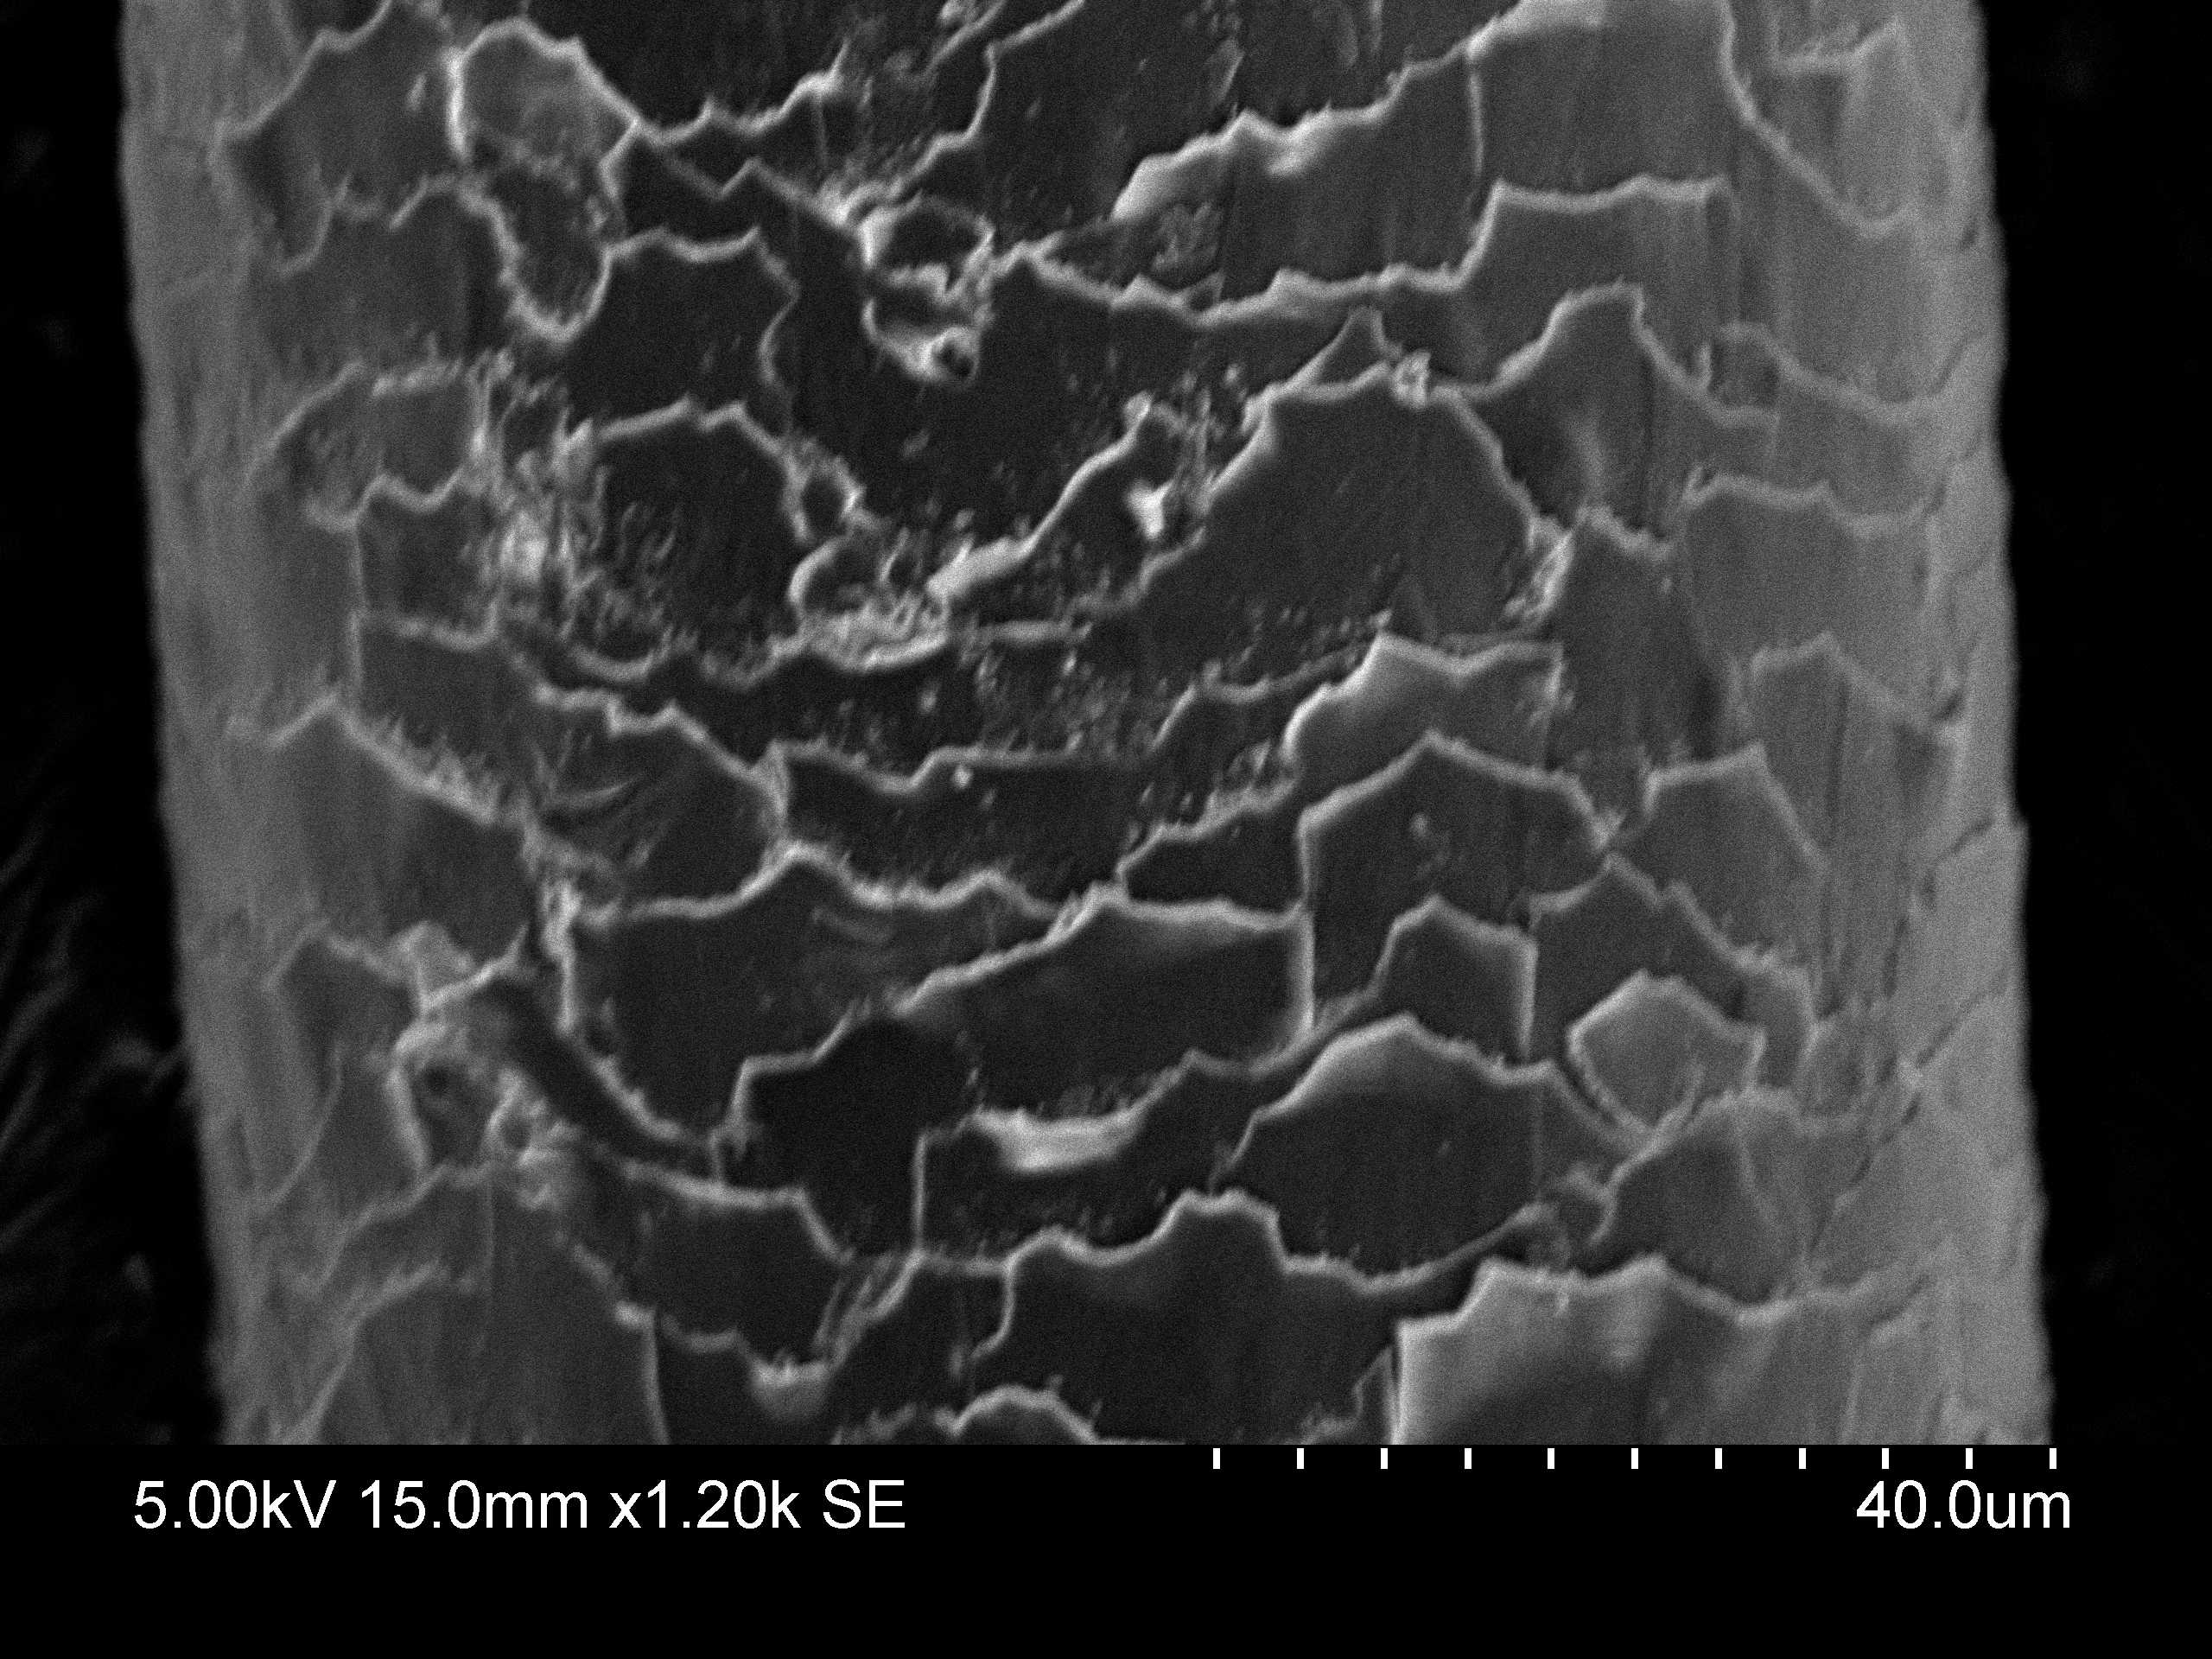
\includegraphics[width = 15cm]{measurements/SE-hair.png}
    \caption{Secondary electron image of human hair}
    \label{fig:se-hair}
\end{figure}
\begin{figure}
    \centering
    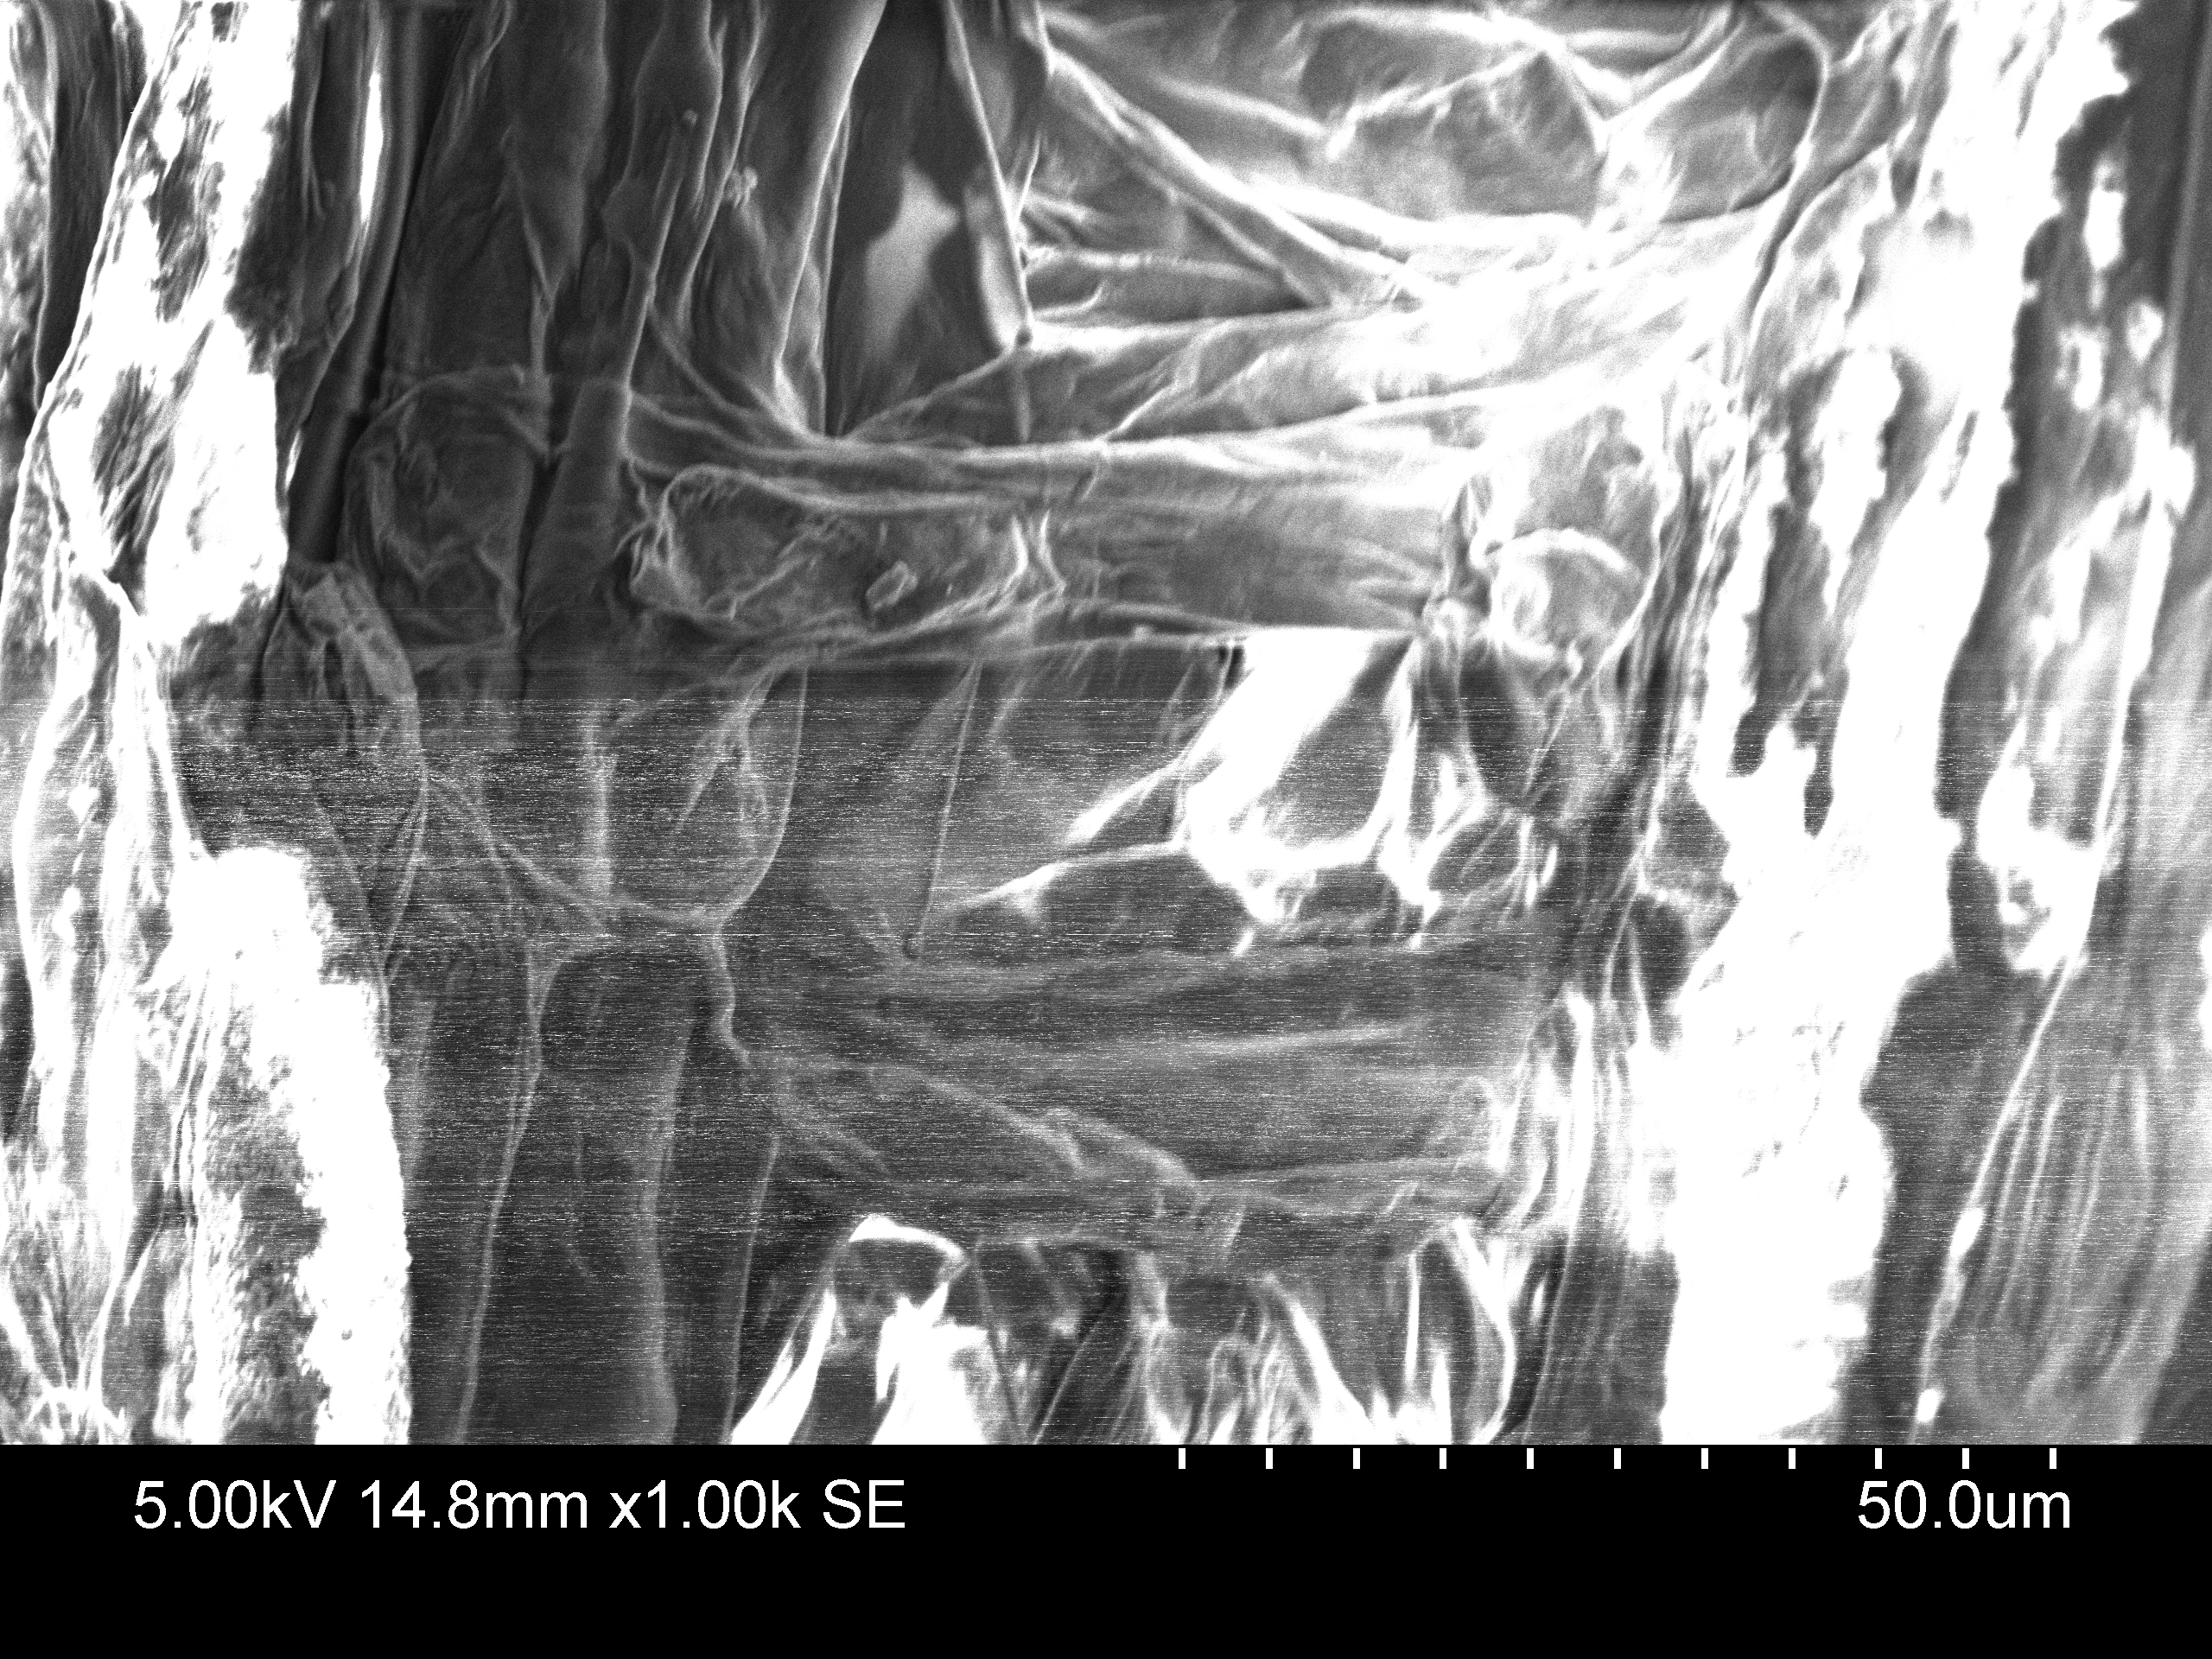
\includegraphics[width = 15cm]{measurements/SE-grass.png}
    \caption{Secondary electron image of grass}
    \label{fig:se-grass}
\end{figure}
\begin{figure}
    \centering
    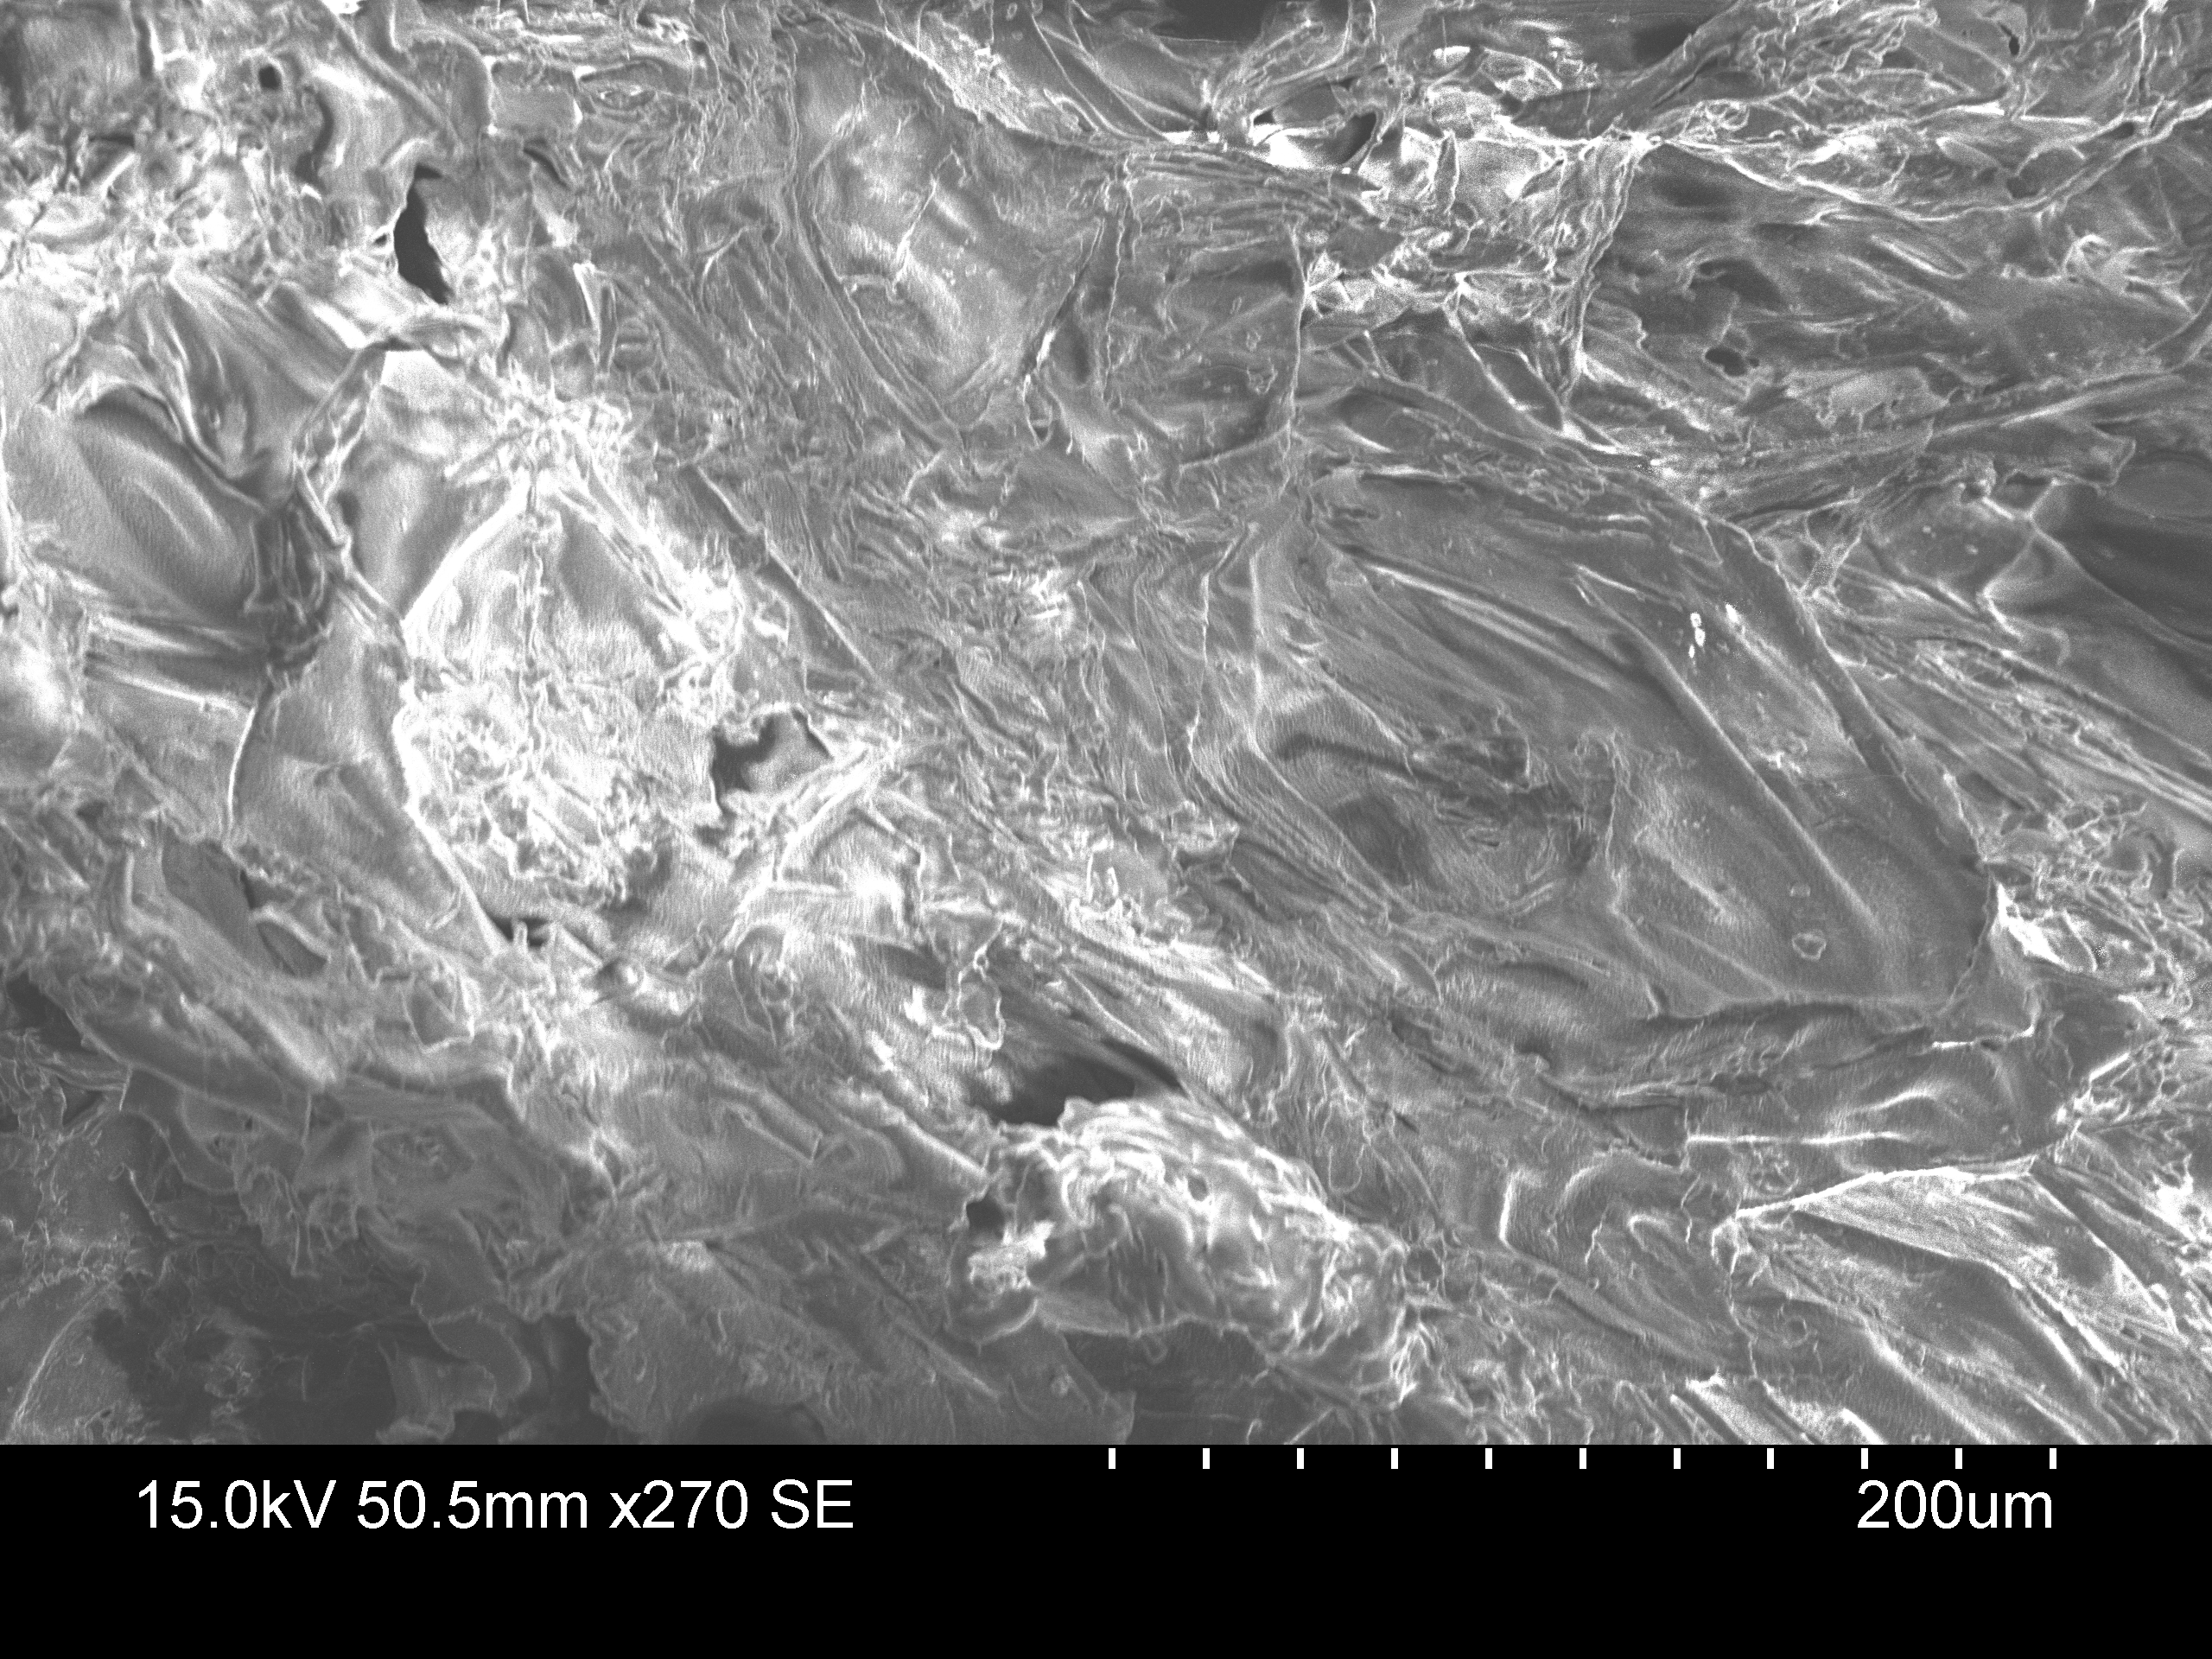
\includegraphics[width = 15cm]{measurements/SE-styro.png}
    \caption{Secondary electron image of styrofoam}
    \label{fig:se-styro}
\end{figure}
\begin{table}
    \centering
    \begin{tabular}{c | c}
    Part & \si{\percent} by atom count \\
    \hline
    Hair & C \SI{77.6 \pm 9.4}{}, O \SI{19.5 \pm 2.8}{}, S \SI{2.69 \pm 0.11}{}, Ca \SI{0.19 \pm 0.02}{} \\
    Grass & C \SI{65.2 \pm 7.8}{}, O \SI{30.1 \pm 4.0}{}, N \SI{2.30 \pm 0.70}{}, K \SI{1.46 \pm 0.05}{}, Cl \SI{0.42 \pm 0.02}{}, Si \SI{0.24 \pm 0.03}{}, S \SI{0.13 \pm 0.02}{}, P \SI{0.06 \pm 0.01}{} \\
    Styrofoam & C \SI{88.1 \pm 9.6}{}, N \SI{6.5 \pm 1.3}{}, O \SI{5.42 \pm 0.91}{}
    \end{tabular}
    \caption{Elemental composition of the other organic samples}
    \label{tab:xr-organic}
\end{table}

Secondary electron images were taken of human hair, some generic lawn grass, and styrofoam, along with their elemental compositions, and can be seen in Figures \ref{fig:se-hair}, \ref{fig:se-grass} and \ref{fig:se-styro}, and Table \ref{tab:xr-organic}.

\section{Discussion}
Since carbon was used as a conductive coating, carbon's presence in all of the elemental analysis is no surprise, but it also means it's numerical value is meaningless.

\subsection{Light Bulb Parts}
\subsubsection{Secondary Electron Images}
Using Figure \ref{fig:se-filament-medium}, one notices seemingly flaky things on the clamped portion of the filament that were not immediately apparent without the magnification. Optical examination revealed the area to be slightly discoloured and duller, possibly indicating oxidation.

In Figure \ref{fig:se-filament-high}, one can clearly see lines on the coils parallel to the direction of the wire. These are likely produced from the manufacturing process, where either the wires are extruded or drawn out from a die, with the lines appearing as the result of imperfections in the die.

The calculated resistance of \SI{63 \pm 12}{\ohm} also matches quite well with the measured \SI{65}{\ohm}. Alternatively, our measured resistivity of \SI{54 \pm 10}{\nano\ohm\metre} matches quite well with the typical value of \SI{52.8}{\nano\ohm\metre} of tungsten.

\subsubsection{Characteristic X-rays}
Oxygen is present in all the metallic components, probably indicating oxidisation, likely during manufacturing since high temperatures during manufacturing would cause faster oxidisation. Alternatively, it could simply be due to organic containments, such as oil from the skin when handling the samples.

The majority of the atoms of the filament is made from tungsten, as expected due to the high melting point requirements of incandescent light bulbs. The small amount of iron probably comes from material left over from the electrode while it was being removed. The sodium is a mystery, however.

The electrode seems to contain a large amount of nickel and iron, which is quite unusual since nickel isn't usually alloyed with iron. When it is, it usually is in the form of stainless steel (with chromium), maraging steel (with cobalt and molybdenum), or nickel cast iron (wouldn't be used for wire-like parts) and even then, there should be more iron than nickel. This along with the presence of sodium is a mystery.

The supports are mostly molybdenum, which is able to withstand high temperatures without softening, along with a high melting point (\SI{2896}{\kelvin}), which is perfect for holding an extremely hot operating light bulb filament in place.

The glass is mostly silicon and oxygen, along with small amounts of sodium, calcium, magnesium and aluminium, typical of soda-lime glass, the most common type (and cheapest) of general-purpose glass. Thus most likely cost was the dominating factor for choosing this glass, since the temperature of the glass during the bulb's operation likely doesn't exceed its glass transition temperature.

The bayonet is mostly iron and zinc, probably indicating it is galvanised iron or steel. Since the bayonet is outside of the bulb, it is prone to oxidisation, hence galvanisation would be a cheap way to prevent it from rusting. The usage of iron or steel would simply be due to its cheapness and hardness, since the point of the bayonet is to hold the bulb in place in its socket.

The contact pad is mostly lead and tin, leading one to believe it is a type of solder. By weight, it would be close to a 90:10 ratio, indicating it might be Sn10 solder. Possible advantages would be that it would be easy to apply a solder during manufacturing, as well as lead solder being quite soft makes it form a good pressure electrical contact with the socket.

\subsection{Copper Grid}
The grid pitch of about \SI{139 \pm 1}{\micro\metre} differs from the manufacturer's value of \SI{125}{\micro\metre}, most likely indicating that the scale calibration on the microscope is slightly off, giving approximately a \SI{11}{\percent} higher value than actual.

The composition of the copper grid is pretty much expected - pure copper.

\subsection{Paper}
Since paper is just fibres pressed together, one expects to see small strands all across the image, and it is in fact what we see, with fibre widths on the order of \SI{10}{\micro\metre}, which is typical for paper. Additionally, many types of paper exhibit grain, where there is a certain direction in which fibres tend to align. Our images are zoomed in too close to see this clearly, but it seems the grain seems horizontal to the image.

As we increase the electron energy, the image seems to loose detail. This is likely due to the electrons penetrating deeper into the sample, and usually the insides of samples have less detail than their surfaces, hence the lower detail.

Additionally, one can see white patches across all three images, increasing in size as energy is increased. These are most likely points where the conductive carbon coating missed, and hence started to become charged up, repelling more electrons and hence creating bright spots.

\subsection{Other Organic Material}
One can clearly see the ``scaly'' nature of hair, as expected.

The long rounded rectangle shaped structures on the grass are probably individual cells of the grass. The white blotchiness and noisiness of the image is likely due to the sample being charged up, and unfortunately limits the detail one can get out of the image.

This is also partly the case with the styrofoam image. Our styrofoam sample was a stretched and twisted sample, so the bubbles one would expect to find styrofoam to be composed of likely have partially popped, explaining the weird detail in the image.

Like one would expect from organic matter, carbon, oxygen and nitrogen dominate the elemental composition. Oddly missing is hydrogen, which may have missed detection due to its rather low energy spectral lines (maximum of \SI{13.6}{\electronvolt}, but detector resolution is of order \SI{100}{\electronvolt}).

The styrofoam should be pure polystyrene, which is simply just carbon and hydrogen. The extra nitrogen and oxygen detected could either be from the air the foam was inflated with (and still trapped inside), or could be from surface containments such as oil from human hands handling the sample.

\end{document}